\documentclass[bibtotoc,liststotoc,BCOR5mm,DIV12]{scrbook}

% use this declaration to set specific page margins
%\usepackage[a4paper , lmargin = {2.7cm} , rmargin = {2.9cm} , tmargin = {2.7cm} , bmargin = {4.6cm} ]{geometry}
\usepackage[a4paper]{geometry}
\usepackage[ngerman, english]{babel}
\usepackage{bibgerm}       		% german references
\usepackage{graphicx} 				% it's recommended to use PDF images but you can use JPG or PNG as well
\usepackage{url}           		% format URLs
\usepackage{hyperref} 				% create hyperlinks
\usepackage{listings, color}	% for source code
\usepackage{subfig}	
\usepackage{multirow}	
\usepackage{makecell}			% two figures next to each other (example: figure 3a), figure 3b)
\usepackage{scrpage2}					% header and footer line
\usepackage{scrpage2}					% header and footer line
\usepackage{array}
\usepackage{xcolor}
\usepackage{pdfpages}
\newcolumntype{L}[1]{>{\raggedright\let\newline\\\arraybackslash\hspace{0pt}}m{#1}}
\newcolumntype{C}[1]{>{\centering\let\newline\\\arraybackslash\hspace{0pt}}m{#1}}
\definecolor{powderblue(web)}{rgb}{0.69, 0.88, 0.9}
\definecolor{silver}{rgb}{0.75, 0.75, 0.75}
\definecolor{lighgray}{rgb}{0.83, 0.83, 0.83}
\lstset{ %
	language=C,                % choose the language of the code
	basicstyle=\footnotesize,       % the size of the fonts that are used for the code
	numbers=left,                   % where to put the line-numbers
	numberstyle=\footnotesize,      % the size of the fonts that are used for the line-numbers
	stepnumber=1,                   % the step between two line-numbers. If it is 1 each line will be numbered
	numbersep=7pt,                  % how far the line-numbers are from the code
	backgroundcolor=\color{lighgray},  % choose the background color. You must add \usepackage{color}
	showspaces=false,               % show spaces adding particular underscores
	showstringspaces=false,         % underline spaces within strings
	showtabs=false,                 % show tabs within strings adding particular underscores
	frame=single,           % adds a frame around the code
	tabsize=1,          % sets default tabsize to 2 spaces
	captionpos=b,           % sets the caption-position to bottom
	breaklines=true,        % sets automatic line breaking
	breakatwhitespace=false,    % sets if automatic breaks should only happen at whitespace
	escapeinside={\%*}{*)} ,         % if you want to add a comment within your code
	commentstyle=\color{blue}
    moredelim=**[is][\color{red}]{@}{@},
}
\lstdefinestyle{base}{
	language=C,
	emptylines=1,
	breaklines=true,
	basicstyle=\footnotesize,
	moredelim=**[is][\color{red}]{@}{@},
}

% header and footer line - no header & footer line on pages where a new chapter starts
\clearscrheadfoot
\ohead{\rightmark}  % comment this line and uncomment the next
% to switch to `chapter name` in the heading
%\ohead{\leftmark}  % comment out to 

\cfoot[\pagemark]{\pagemark}
\cfoot[\pagemark{} of \pageref{LastPage}]% for pagestyle `scrplain`
{\pagemark{} of \pageref{LastPage}}% for pagestyle `scrheading`

% set path where images are stored
\graphicspath{{./img/}}

%
% der Befehl \hypenation versteht keine Sonderzeichen, also weder �
% noch "a noch \"a. W�rter die derartige Zeichen enthalten m�ssen
% direkt im Text getrennt werden, z.B. W�r\-ter
%
\hyphenation{te-le-com-muni-cation 
te-le-com-muni-cation-specific 
Te-le-kom-mu-ni-ka-tions-API} 					% use this file to set explicit hyphenations (doesn't seem to work correctly)

\begin{document}
	
% ---------------------------------------------------------------
\frontmatter
    \thispagestyle{empty}
\begin{center}

\vspace*{1.4cm}
{\LARGE \textbf{Technische Universit�t Berlin}}

\vspace{0.5cm}

{\large Fakult�t Elektrotechnik und Informatik\\[1mm]}
{\large Institut f�r Softwaretechnik und Theoretische Informatik\\[5mm]}
{\large Security in Telecommunications\\[5mm]}


Fakult�t IV\\
Sekr. TEL17 \\
Ernst-Reuter-Platz 7 \\
10587 Berlin\\
http://www.eecs.tu-berlin.de\\

\vspace*{1cm}


\includegraphics[width=4cm]{tu_logo.jpg}

\vspace*{1.0cm}

{\LARGE Master Thesis}\\

\vspace{1.0cm}
{\LARGE \textbf{Porting the Xen Emulation Layer}}\\
\vspace*{0.3cm}
{\LARGE \textbf{to static hypervisor}}\\
\vspace*{1.0cm}
{\LARGE Amna Waseem}
\\
\vspace*{0.5cm}
Matriculation Number: 387424\\
01.11.2017\\ % 	date of submission


Supervised by\\
Prof. Dr. Jean-Pierre Seifert\\
Assistant Supervisor\\
Dr.-Ing. Jan Nordholz and Robert Buhren 
\vspace{3cm}


\end{center}


   	\thispagestyle{empty}
    \cleardoublepage
    
   % \chapter*{Acknowledgments}

I would like to thank Robert Buhren for giving me this opportunity to work on a very exciting topic for my Master Thesis and introducing me to a new challenging domain of virtualization. The door to his office was always open whenever I ran into a problem or had any questions related to research. He had allowed me to work independently on designing implementation strategies of research, but guided me in the right direction whenever he thought I needed it. I also want to thank everybody at Security in Telecommunications group at TU Berlin for the wonderful time, especially, Jan Nordholz for sharing his wisdom and answering all my questions. 

   % \thispagestyle{empty}
   % \cleardoublepage
    
    %\newpage

\thispagestyle{empty}

\begin{large}

\vspace*{6cm}

\noindent
Hereby I declare that I wrote this thesis myself with the help of no more than the mentioned literature and auxiliary means.
\vspace{2cm}

\noindent
Berlin, 01.01.2050

\vspace{3cm}

\hspace*{7cm}%
\dotfill\\
\hspace*{8.5cm}%
\textit{(Signature [your name])}

\end{large}
 
    %\thispagestyle{empty}
    %\cleardoublepage
    
    
    \thispagestyle{empty}
\vspace*{1.0cm}

\begin{center}
    \textbf{Abstract}
\end{center}

\vspace*{0.5cm}

\noindent
Over the past decade, virtualization technologies have gone from server consolidation in corporate data centers to small forms of embedded platforms for providing system security, hardware isolation, resource management and I/O device emulation. With the modern computers providing different forms of I/O devices, there has been huge development in hypervisors' technology to provide efficiency in the use of physical resources. Major hypervisors in virtualization market have been continuously deploying different memory techniques to dynamically allocate memory and use resources more efficiently. However, this dynamicity in memory allocation introduces difficulty in provabilty and verification of configured hypervisor used in safety critical applications. PHIDIAS, a static hypervisor developed by Security in Telecommunications department of Elektrotechnik und Informatik faculty at Technischen Universit�t Berlin, is built around the concept of Principle of Staticity to ease provability and reduce runtime complexity along with memory footprint by eliminating dynamic elements from the system. However, it does not have support of I/O device emulation. In this thesis, Xen Hypervisor's I/O device framework has been ported to PHIDIAS using existing mechanisms of static memory sharing and inter-guest communications.

    \thispagestyle{empty}
    \cleardoublepage
    
  %  \thispagestyle{empty}
\vspace*{1cm}

\begin{center}
    \textbf{Zusammenfassung}
\end{center}

\vspace*{0.5cm}

\justify

In den letzten zehn Jahren sind Virtualisierungstechnologien von der Serverkonsolidierung in Unternehmens-Datenzentren hin zu kleinen Formen von eingebetteten Plattformen f�r Systemsicherheit, Hardwareisolierung, Ressourcenverwaltung und E / A-Ger�teemulation gegangen. Mit den modernen Computern, die verschiedene Formen von I / O-Ger�ten bereitstellen, hat es eine enorme Entwicklung in der Hypervisor-Technologie gegeben, um eine Effizienz bei der Verwendung von physischen Ressourcen bereitzustellen. Gro�e Hypervisor-Anbieter im Virtualisierungsmarkt haben kontinuierlich verschiedene Techniken entwickelt, um Speicher dynamisch zuzuweisen und Ressourc-
en effizienter zu nutzen. Diese Dynamizit�t bei der Speicherzuweisung f�hrt jedoch zu Schwier-igkeiten bei der Verifizierung und Verifizierung des konfigurierten Hypervisors, der in sicherheitskritischen Anwendungen verwendet wird. PHIDIAS (Proviable Hypervisor mit Integrated Deployment Information und Allocated Structures) ist ein statisch konfigurierter Hypervisor, der von der Abteilung Sicherheit in der Telekommunikation der Fakult�t f�r Elektrotechnik und Informatik der Technischen Universit�t Berlin entwickelt wurde und das Prinzip der Statik zur Erleichterung der Beweisbarkeit und zur Reduzierung der Laufzeitkomplexit�t beinhaltet. mit reduziertem Speicherbedarf durch Eliminierung dynamischer Elemente aus dem System. Die E / A-Ger�tevirtualisierung wird jedoch nicht unterst�tzt. In dieser Arbeit wurde das I / O-Device-Framework von Xen Hypervisor unter Verwendung der vorhandenen Mechanismen der statischen Speicherfreigabe und der Inter-Guest-Kommunikation nach PHIDIAS portiert. Das Arbeiten und Testen von portierten virtualisierten Netzwerkger�ten wurde gezeigt. Die Ergebnisse werden gesammelt, um den Durchsatz und die Bandbreite virtueller Netzwerkschnittstellen bei nativem Xen- und PHIDIAS-Setup zu vergleichen. Die Ergebnisse unterstreichen die Tatsache, dass PHIDIAS eine bessere Leistung f�r Pakete ohne Fragmentierung liefert, indem die Hypervisor-Schicht zur Behandlung von Xen-spezifischen Hypercalls umgangen wird. Der aktuelle Ansatz bei portierten Netzwerktreibern f�hrt jedoch zu einem Overhead, w�hrend fragmentierte Pakete manuell kopiert werden, da PHIDIAS kein Hypercall implementiert hat, um gemeinsam genutzte Seiten in den Gastdom�nenbereich zu mappen, indem entsprechende Seitentabelleneintr�ge im Vergleich zu Xen modifiziert werden.
\\
\\
\keywords{I/O-Virtualisierung, Hypervisor, Xen, statische Konfiguration, ARM-Architektur}\\

   % \thispagestyle{empty}
    
    
    \tableofcontents
    \thispagestyle{empty}
    
    \listoffigures
    \thispagestyle{empty}
    
    \listoftables
    \thispagestyle{empty}
    
% --------------------------------------------------------------

\mainmatter % comment single chapters for faster compilation

    \chapter{Introduction\label{cha:chapter1}}

In this section, a brief introduction of virtualization and hypervisor technologies will be given. A little comparison of Xen, KVM and Phidias will be provided as well.

\section{Motivation\label{sec:moti}}

In this section, motivation behind adding device I/O emulation support in Phidias will be discussed e.g. to prove flexibility of a static hypervisor and to ease provability. This section will also highlights the reasons for choosing Xen as a reference.

\section{Objective\label{sec:objective}}

This section will describe the problems and issues which will be solved in this thesis. The main aim of this thesis will be given in this section e.g using existing Phidias memory sharing and IPI mechanism to port Xen Split Driver model for I/O virtualization and keep changes as minimal as possible.

\section{Scope\label{sec:scope}}

In this section, method for porting device I/O emulation of Xen to Phidias will be discussed i.e. main approach will be discussed to port split driver model to Phidias. 

\section{Outline\label{sec:outline}}

This section gives a brief introduction into the main chapters. 
\\
\\
\noindent This example thesis is separated into 7 chapters.
\\
\\
\textbf{Chapter \ref{cha:chapter2}} is called 'Background'. Here I will give background information to lay foundation of thesis topic.
\\
\textbf{Chapter \ref{cha:chapter3}} provides the requirements and assumptions of thesis
\\
\\
\textbf{Chapter \ref{cha:chapter4}} discussed  'Design' and 'Model'. Here I will describe my approach, give a high-level description to the architectural structure and to the basic components that my design consists of.
\\
\\
\textbf{Chapter \ref{cha:chapter5}} describes the implementation part of my work.
\\
\\
\textbf{Chapter \ref{cha:chapter6}} is 'Evaluation'. How the testing is performed for thesis will be discussed. Measurements, tests, screenshots will be included.
\\
\\
\textbf{Chapter \ref{cha:chapter7}} summarizes the thesis, describes the problems that occurred and gives an outlook about future work.
    \chapter{Background \label{cha:chapter2}}

In order to set context of underlying work of thesis, this section provides background information on virtualiaztion technologies and embedded systems with special emphasis on the ARM platforms. A brief overview of Phidias, a static hypervisor in question is also given in this section.
\section{Introduction to Virtualization \label{sec:tech}}
Virtualization is a mechanism of providing abstraction between computer hardware systems and softwares running on them, allowing us to create multiple computing environments exploiting the resource isolation on a single physical platform. It basically gives a logical view of multiple operating environments running on a single hardware. With the recent developments in virtualization, there has been huge investments in organizations over this technology to improve the efficiency and availability of resources and applications. Enterprises are giving up the old \textbf{one server, one application} model and gaining benefits from server consolidation provided by virtualization. Virtualization has dramatically changed the IT landscape by reducing its expenses and providing economies of scale and greater efficiency.

\subsection{History of Virtualization\label{sec:history}}
History of virtualization dates back to 1950's when the Compatible Time Sharing System (CTSS) was developed at MIT on IBM 704 series computer. The supervisor program of CTSS handled console I/O, scheduling of foreground and background (offline-initiated) jobs, temporary storage and recovery of programs during scheduled swapping, monitor of disk I/O, etc. The supervisor had direct control of all trap interrupts \cite{introtousevirtualization}.\\
\\
In the fall of 1963, MIT's Project MAC was founded with the main purpose of designing and implementation of a better time sharing system than CTSS. After IBM lost the bid to General Electric's GE 645, it created a number of virtual machine systems e.g, the CP-40 (developed for a modified version of IBM 360/40), the CP-67 (developed for the IBM 360/67), VM/370, and many more. We can roughly say that Virtual Machine technology was brought to users with the introduction of the CP-67 hypervisor on the S/360 Model 67 processor. In 1999, VMware introduced virtualization on x86 platforms. Since then, many vendos like Microsoft, Citrix etc had followed VMware and technology has been evolved with the advances in hardware architectures. 
\\
\\
\subsection{Benefits of Virtualization\label{sec:uses}}
For many years, server virtualization was considered one of the biggest advantages of using virtualization technology and VMware enjoyed a long run as king of x86 server virtualization. However, many players e.g. Citrix and Microsoft started to gain ground in this field by providing additional middleware and desktop virtualization offerings. Over the past several years, there has been huge deployments in virtualization and vendors are continuously innovating to increase virtualization capabilities of systems and developing management tools.\\
\\
There are many advantages of using virtualization technology. Following are some of the main benefits due to which virtualization has become a mainstream tool in the computing industry \cite{reasonstousevirtualization}:


\subsubsection{Better utilization of resources \label{sec:resource optimization}}
With virtual machines, resources of computing platforms can be used in an optimal manner to achieve better performance. Servers used in data centers typically have large resource capabilities. However, they are not fully utilized because of small number of connected users or less demanding applications. Virtualization of hardware allows on-demand resource allocation leading to efficient use of computing power, storage space and network bandwidth. In addition to on-demand usage of resources, virtualization also provides resource isolation between virtual machines. Each virtual machine can run software without affecting others code execution. 

\subsubsection{Consolidation \label{sec:Consolidation}}
For many years, individual servers have been dedicated to run single applications. For less demanding applications, computing capabilities would be wasted. With the advent of virtualization, organizations are now deploying several applications on single servers using only a small amount of processing power. Server consolidation has led to dramatic reduction in need of floor space, HVAC, A/C power, and co-location resources which has caused cost reduction and efficient power consumption.

\subsubsection{Security and Isolation\label{sec:security}}
Virtualization allows running multiple virtual machines in an isolated secure environment. All privileged calls made by guests' kernels are analyzed by hypervisor to provide safety against vulnerabilities and attacks. Exceptions and traps of one virtual machine are handled by hypervisor layer isolating other virtual machines from the resulting affects. Virtualization regulates access permissions to programs with reduced privileges from misusing resources. 

\subsubsection{Migration and Increased Uptime\label{sec:migration}}
Migration is the process of moving a running virtual machine from one place to another without affecting overall system. With virtualization, organizations can get better performance and reliable systems. It also increases uptime of servers and applications. Virtual machines can easily be backed up and restored for speedily recovery from computing disasters.


\subsection{Overview of Hypervisors\label{sec:aaa}}

A virtualization layer that separates the service request from underlying physical delivery of that request is called virtual machine monitor (VMM) or hypervisor. Hypervisor allows multiple operating systems to run concurrently within virtual machines on a single computer and provides dynamic allocation and sharing of physical resources e.g. CPU, memory, storage and I/O devices \cite{hypervisor1}.Hypervisor enables communication between hardware
and a virtual machine so that the virtualization accomplishes with this abstraction layer (hypervisor) \cite{hypervisor2}.  Figure \ref{Virtualization} shows the virtual machine abstraction architecture.

\begin{figure}[htb]
\centering
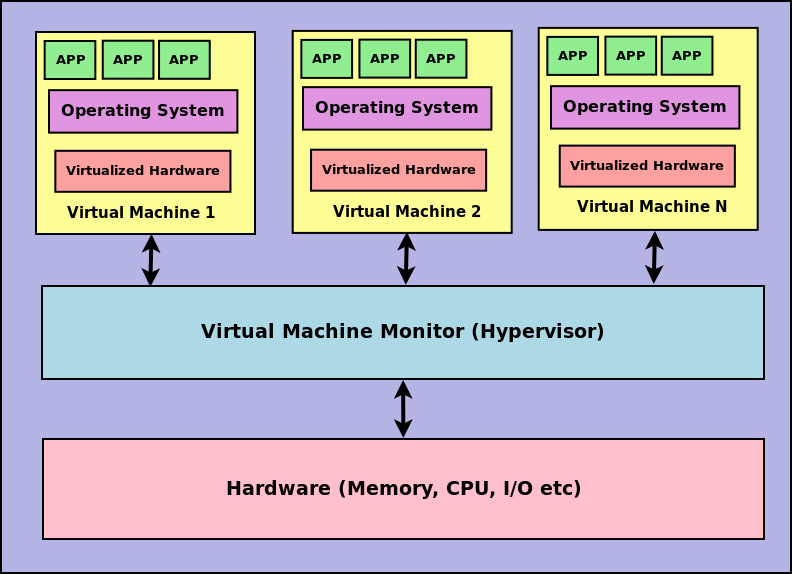
\includegraphics[width=10cm]{Virtualization_Abstraction}
\caption{Virtualization Framework}
\label{Virtualization}
\end{figure}
In 1974, Popek and Goldberg described the requirements of a hypervisor for efficient virtualization in the article `Formal Requirements for Virtualizable Third Generation Architectures' \cite{popek_goldberg_1973}. There are three requirements to be fulfilled by hypervisors:
\begin{itemize}
	\item Virtualization environment provided by hypervisor should be native system so that program behaves in a similar fashion.
	\item Virtualized resources should be shared with security controls to protect from any threats and performance interference.
	\item Good support to handle privileged instructions should be provided in order to avoid performace degradation.
\end{itemize}
Keeping in view the above requirements, different types of hypervisors have been introduced in market with different implementation level of virtualization which will be described in next sections.

\subsection{Types of Hypervisors\label{sec:bbb}}
There are two basic types of hypervisors i.e. Type 1 and Type 2 Hypervisors as shown in Figure \cite{Hyper1vsHyper2}.
\begin{figure}[htb]
	\centering
	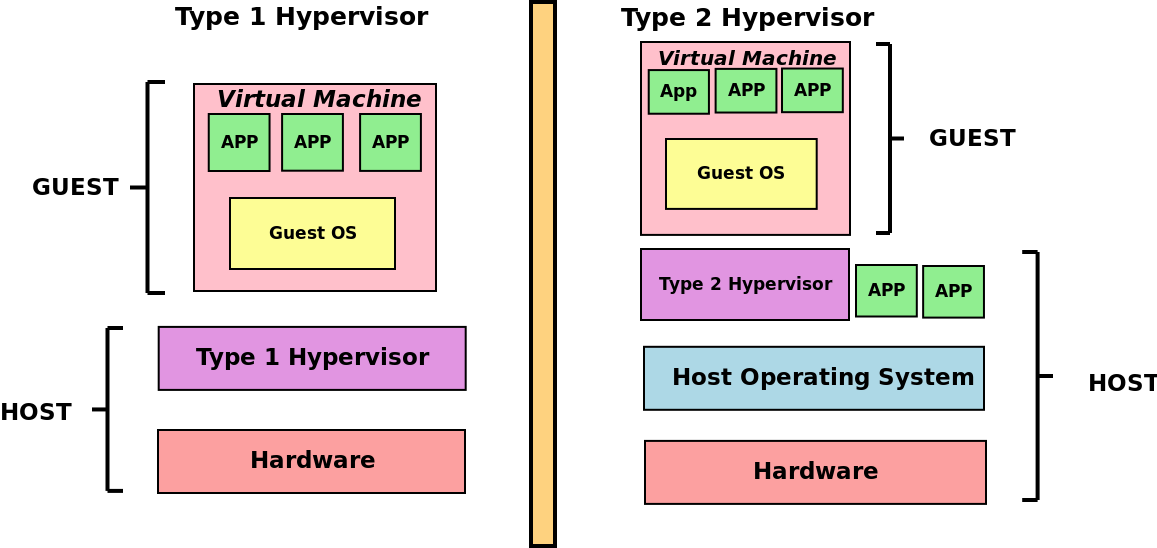
\includegraphics[width=10cm]{Hyper1vsHyper2}
	\caption{Type1 Hypervisor vs Type 2 Hypervisor}
	\label{Virtualization}
\end{figure}
%\newpage
\begin{itemize}
	\item \textbf{Type 1} hypervisor sits directly on hardware and manages virtual machines on top of it. It is also called bare-metal hypervisor. Examples of type 1 hypervisors are VMware vSphere/ESXi, Microsoft Windows Server 2012 Hyper-V, Citrix XenServer, Red Hat Enterprise Virtualization (RHEV) and open-source Kernel-based Virtual Machine (KVM) \cite{hypervisor2}.
	\item \textbf{Type 2} hypervisor runs on host operating system to manage virtual machines here hosted operating system provides hardware configuration.  VirtualBox and VMware
	Workstation are examples of type 2 hypervisors.
\end{itemize}
According to IBM, Type 1 hypervisors provide higher performance, availability, and security than Type 2 hypervisors.IBM recommends that Type 2 hypervisors be used mainly on client systems where efficiency is less critical or on systems where support for a broad range of I/O devices is important and can be provided by the host operating system \cite{searchservervirtualization}.
\\
Since bare-metal hypervisor has direct access to the hardware resources rather than going through
an operating system, it is considered to be more efficient than a hosted architecture and delivers greater scalability, robustness and performance \cite{hypervisor1}. 

\subsection{State of the Art Hypervisors\label{sec:comp}}
Over the past decade, virtualization technology has gone from small deployments to full blown IT infrastructure development. Technology makers have shifted their focus from operating systems with one-to-one relationships with hardware to virtualized approaches to shared resources among multiple operating systems on one hardware. When we talk about virtualization players in market, VMware is the first one which comes to our mind. Besides VMware, now other players like Citrix XenServer, Microsoft Hyper-V,Red Hat Enterprise Virtualization (RHEV), Oracle's Solaris Zones, LDoms and xVM, Amazon's Elastic Compute Cloud (EC2), Google Ganeti cluster virtual server management software tool and Virtual Bridges' VERDE product \cite{players} have entered this new market and are continuously developing innovation virtualization solutions to meet specific requirements of different industries. In 2011, Younge, Andrew J., et al. \cite{younge2011analysis} compared several virtualization technologies which is provided in Figure \ref{comparison}.
\begin{figure}[!htbp]
	\centering
	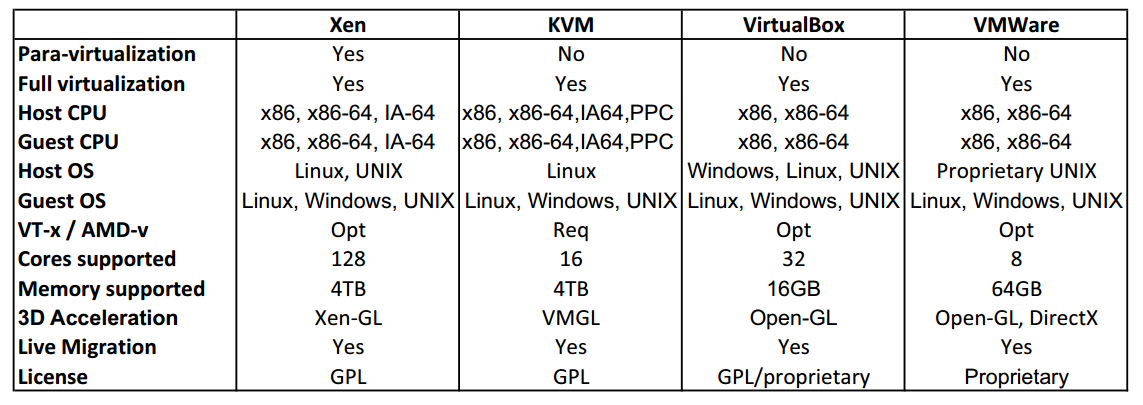
\includegraphics[width=10cm]{Comparison}
	\caption{A comparison chart between Xen, KVM, VirtualBox, and VMWare ESX. Adapted from from "Analysis of virtualization technologies for high performance computing environments" by Younge, Andrew J., et al, 2011, p11}
	\label{comparison}
\end{figure}

\section{Embedded Systems \label{sec:standard}}
Embedded systems are composed of simple devices used to perform small and dedicated functions with specific hardware and software constraints like low memory and efficient power usage, more battery life, smaller code footprint, smaller size and weight with reduced cost and reliability \cite{koopman1990design}. According to Steve Heath \cite{heath_2005}, an embedded system is a microprocessor-based system that is built to control a function or a range of dedicated functions and is not designed to be programmed by the end user in the same way as general purpose PC is. He had described several features of embedded systems which had led to the wide spread use of microprocessors in industry. Some of main features are as follows:
\begin{itemize}
	\item \textbf{Replacement of discrete logic circuits} to reduce the time and cost of developing new products by changing program code to process data in embedded systems.
	\item \textbf{Upgrading systems} by changing the software while keeping the hardware same thus reducing the cost of production and testing of software.
	\item \textbf{Providing easy maintenance upgrades} for adding new functionalities and resolving bugs by reprogramming the software without modifying the hardware.
	\item \textbf{Protecting intellectual property} by encapsulating the functionality of system by burning firmwares on chips making it harder to reverse engineer it.
\end{itemize}
In order to better understand embedded systems, we can look at differences from general purpose computers. General purpose computers are developed to run all types of general applications. However, embedded systems are designed for a fixed or a few number of dedicated functions. General purpose computers are reprogrammable by end users while embedded systems are not reprogrammable by end users. Embedded systems are smaller in size and run at fixed optimized speed for a specific purpose while general purpose computers are bigger in size with speed which does not need to be always predictable but faster is always better.
\\
\\
Embedded systems, once used only for single purpose time critical applications, are now becoming important for all devices used in our everyday life. Such devices are now able to run general purpose operating systems or application with little or no knowledge of hardware constraints. Although safety critical systems are far more restricted that so-called modern embedded systems, virtualization could bring advantages, by increasing their safety, reliability and security \cite{aguiar_hessel_2010}.

\subsection{Virtualization on Embedded Systems\label{sec:itu}}
 Adding a hypervisor to an embedded system adds flexibility and higher-level capabilities, morphing the embedded device into a new class of system \cite{ibm}. Embedded devices are ubiquitous and are major part of our lives today. Their common use is in real time applications with hardware and software constraints. But why there is a trend seen today to use these devices in virtualized systems. One of the reasons is that users now want to run applications developed originally for general purpose OSes and still desire to achieve real time responsiveness. There is where virtualization comes in handy. With virtualization, we can enable concurrent execution of real time OS (RTOS) and application OS(Windows, Linux etc) on same hardware. Another benefit will be security which can be achieved by encapsulating vulnerable application OS in a separate VM thus preventing access to the rest of the system.
 \\
 \\
 In a nutshell, there are many uses of deploying virtualization on embedded systems and with the development in multi-cores technology, we can expect innovative solutions in future embedded virtualized platforms. 

\subsection{ARM Embedded Platforms\label{sec:itu}}
Since the processor used in thesis is ARMv8 Cortex-A53, a brief introduction of ARM architecture in general and ARMv8 in specific along with its features will be provided in this section.
\subsubsection{Introduction to ARM Architecture\label{sec:arch}}
ARM, originally \textbf{Acorn RISC Machine}, later \textbf{Advanced RISC Machine}, is a family of reduced instruction set computing (RISC) architectures for computer processors, configured for various environments \cite{wikipedia_2017}. ARM has the following RISC architecture features \cite{ARM}:
\begin{itemize}
	\item A uniform register file load/store architecture, where data processing operates only on register contents, not directly on memory contents. 
	\item Simple addressing modes, where all load/store addresses are only determined from register contents and instruction fields.
\end{itemize}
With the increase in demands of new functionality and emerging market trends, ARM architecture has evolved over time. It has introduced the concept of \textbf{profiles} which define different versions of the architecture used for different types of processors which are aimed to to used in different market segments \cite{ARM}. Table \ref{tableARM} shows these different profiles of ARM architecture.
\begin{table}[!htbp]
\centering
\begin{tabular}[t]{|L{4cm} |L{8cm}|}
\hline
Profile & Description \\
\hline
Architecture (`A') profile  & Provides high performance and 
usually used in mobile and enterprise markets  \\
\hline
Real-Time (`R') profile & Provides real time performance and
 used in embedded applications for automotive and industrial control. \\
\hline
Microcontroller (`M') profile & Provides time critical and  real time performance for microcontroller market\\
\hline
\end{tabular}
\caption{Description of ARM profiles}
\label{tableARM}
\end{table}
ARM processors are basically used to achieve high-performance at lower cost with efficient power consumption.

\subsubsection{ARM processor modes and Registers\label{sec:processor_modes}}
There are two categories of ARM processor modes i.e. privileged  and non-privileged modes. Privileged mode is used to handle exceptions or to access system resources while non-privileged mode has restricted access to protected resources. Each processor mode uses a its own stack and a subset of registers. Table \ref{tab:modes} shows different processor modes supported by ARM architecture.
\begin{table}[!htbp]
	\centering
	\begin{tabular}[t]{|L{3cm} |L{8cm}|C{2cm}|}
		\hline
		\multicolumn{1}{|c|}{\textbf{Modes}}  &	\multicolumn{1}{|c|}{\textbf{Description}}    & 	\multicolumn{1}{|c|}{\textbf{Category }  }    \\ 
		\hline

		User                 & Normal program execution  & Privileged  \\\hline

		Fast interrupt (FIQ) & Handles fast interrupts  &     \\
        \cline{1-2}
		Interrupt (IRQ)      & Handles regular interrupts  &      \\
\cline{1-2}
		Supervisor           & Handles operating system functions. System enters into this mode when the power is applied.     &    \multirow{5}{*}{\centering Privileged}   \\
\cline{1-2}
		Abort                & Handles Data Aborts and Prefetch Aborts and helps to implement virtual memory        &      \\
\cline{1-2}
		System               & Handle operating systems function  in user mode and uses same registers as User mode    &      \\
\cline{1-2}
		Undefined            & Handles Undefined instructions with the support of software emulation of hardware co-processors &     \\
		\cline{1-2}
		Monitor & Provides support of switching between secure and  non-secure states available on processors with security extensions & \\
			\hline
	\end{tabular}
	\caption{Description of ARM processor modes}
	\label{tab:modes}
\end{table}
In all ARM processors, the following registers are available and accessible in
any processor mode \cite{arm_information_center}:
\begin{itemize}
	\item 13 general-purpose registers R0-R12
	\item 1 Stack Pointer (SP)
	\item 1 Link Register (LR)
	\item 1 Program Counter (PC)
	\item 1 Application Program Status Register (APSR)
\end{itemize}
ARM processor has total of 37 registers (40 with security extension implementations) arranged in partially overlapping banks which help to context switch rapidly. Figure \ref{ARM_Registers} shows the organization of general purpose registers of different ARM processor modes.


\begin{figure}[!htbp]
	\centering
	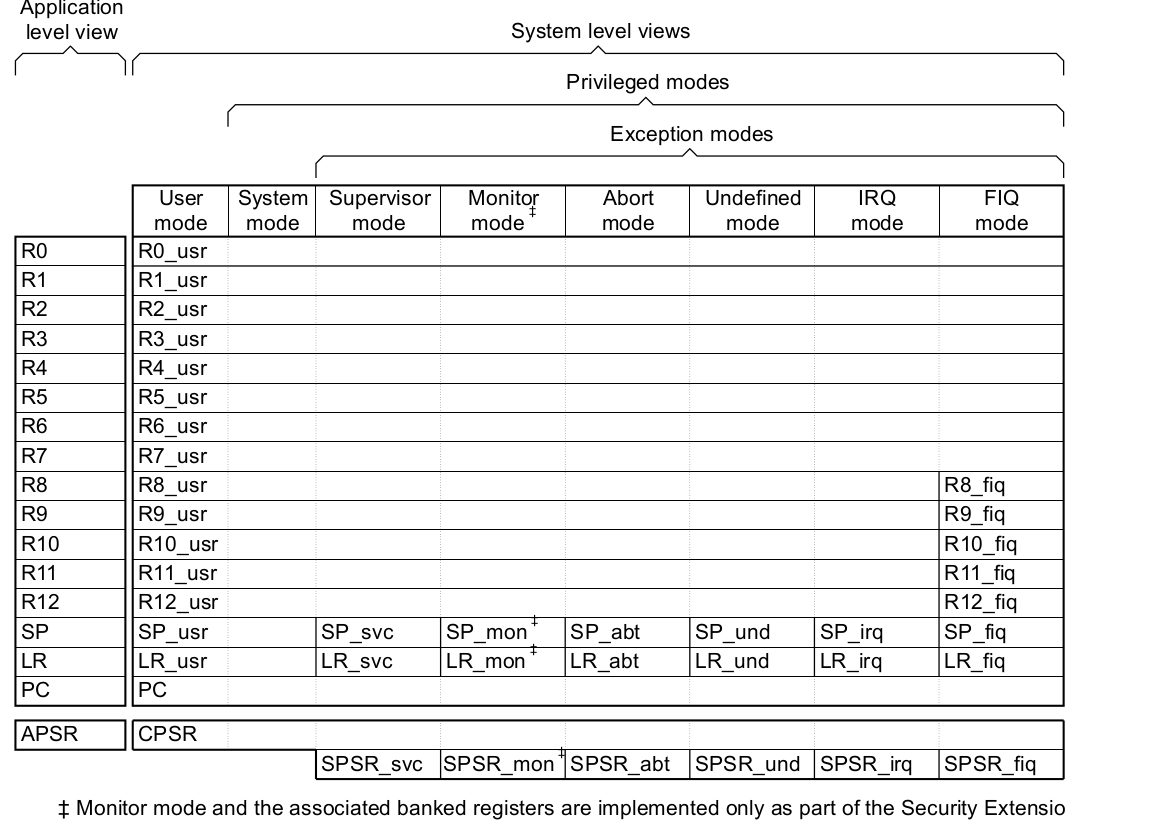
\includegraphics[width=10cm]{ARM_Registers}
	\caption{Organization of ARM registers for different processor modes. Taken from \cite{arm_information_center}}
	\label{Virtualization}
\end{figure}
\subsection{ARMv8-A Architecture\label{sec:armv8}}
The basic feature of ARMv8 architecture is that it supports both 32-bit (AArch32) and 64-bit (AArch64) execution states.For AArch64 state, addresses are placed in 64-bit registers and instructions can use 64-bit registers for processing while on the other hand, AArch32 allows instructions to use 32-bit registers  and addresses are placed in 32-bit registers \cite{armv8}. For this thesis, AArch64 execution state has been used which supports up to four Exception levels, EL0 - EL3 and has 64-bit virtual addressing. Table \ref{exeception_model} shows the description of exception model levels.
\begin{table}[!htbp]
	\centering
	\begin{tabular}[t]{|L{4cm} |L{8cm}|}
		\hline
		Exception Level & Description \\
		\hline
		 EL0 &  Applications\\
		\hline
		EL1 & OS kernel and associated privileged functions \\
		 \hline
		 EL2& Hypervisor  \\
		 \hline
		 EL3 &  Secure Monitor\\
		 \hline
	\end{tabular}
	\caption{Description of ARMv8 Exception Model Levels}
	\label{exeception_model}
\end{table}
The Cortex-A53 processor is a mid-range, low-power processor that implements the ARMv8-A
architecture with  Generic Interrupt Controller (GIC) v4 and ARM Generic Timer  \cite{cortexA53}.
\subsubsection{ARMv8-A Memory Management\label{sec:armv8_mem}}
Memory memory unit (MMU) is a hardware that performs virtual address to physical address mapping. It does this by controlling table walk hardware which accesses translation tables held in main memory.Transalation tables hold virtual to physical address mappings and memory attributes which are then loaded into the Translation Lookaside Buffer (TLB) when a location is accessed \cite{cortexA53}.
With MMU enabled in system, applications can run independently in their own virtual address space without having the knowledge of physical addresses used by hardware. Figure \ref{mmu} shows the MMU hardware in ARM architecture.
\begin{figure}[!htbp]
	\centering
	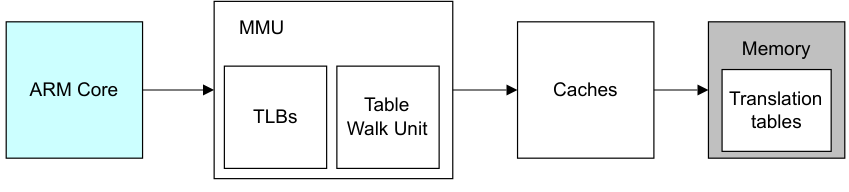
\includegraphics[width=10cm]{mmu}
	\caption{Organization of ARM registers for different processor modes. Taken from \cite{mmu}}
	\label{mmu}
\end{figure}

For ARMv8 hardware used in thesis, 48-bit virtual address with 4KB granule size has been used. Cortex-A53 processor uses a four level address lookup with 4KB page size. The 48-bit address has nine bits for each level of translation with the last 12 bits of original address defining the offset within the 4kB page size. Each level of translation lookup table has 512 entries.
Bits 47:39 of the Virtual Address index into the 512 entry L0 table. Each of these table entries spans a 512 GB range and points to an L1 table. Within that 512 entry L1 table, bits 38:30 are used as index to select an entry and each entry points to either a 1GB block or an L2 table. Bits 29:21 index into a 512 entry L2 table and each entry points to a 2MB block or next table level. At the last level, bits 20:12 index into a 512 entry L2 table and each entry points to a 4kB block \cite{translation}. Figure \ref{translation} shows the division of 48 bit address for four levels of translation lookup used for 4KB granule size by MMU.

\begin{figure}[!htbp]
	\centering
	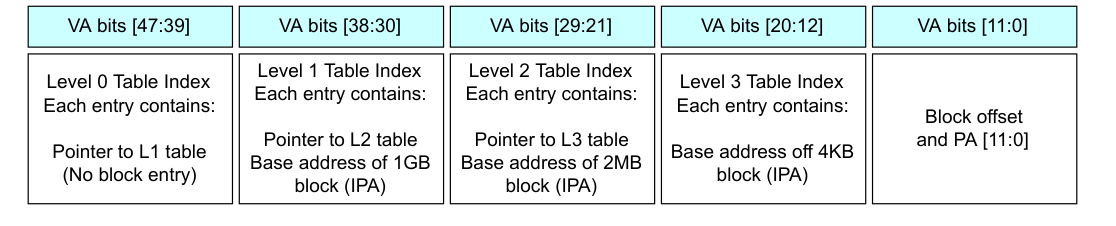
\includegraphics[width=10cm]{translation}
	\caption{48-bit address translation lookup for 4KB granule size on ARMv8 architecture. Taken from \cite{translation}}
	\label{translation}
\end{figure}


\subsection{Device Emulation on ARMv8-A Embedded Systems\label{sec:3gpp}}
ARMv8-A architecture supports virtualization by implementing EL2 execution state for running hypervisor. Hypervisor in EL2 state is responsible for running multiple guests in non-secure EL1 state. Each guest can run applications in non-secure EL0 state. Address translation occurs in two stages in case of running virtualized guest operating systems. Stage 1 translation converts virtual addresses to intermediate physical address (IPA) which is managed by Guest OS in EL1 state. Stage 2 translation converts IPA to physical address which is managed by hypervisor in EL2 state. These IPA are treated as actual physical addresses by Guest OS. ARM virtualization extensions has made generic timers and the GIC interrupt controller virtualization aware. Hence CPU, memory, interrupts and timers can be emulated using full hardware virtualization. However, for I/O devices, para-virtualized drivers could be used.\\
\\
On ARM architecture, device virtualization can be done using memory mapped devices. All reads/writes to devices gets trapped by hypervisor which should be capable of emulating device loads/stores. With ARM virtualization extensions, device virtualization has become more efficient. The main features of these extensions include  introduction of a new higher privileged Hypervisor execution mode than Supervisor mode, mechanisms to aid interrupt handling and the provision of a System MMU to aid memory management, supporting: multiple translation contexts for multiple DMA capable masters, two levels of address translation and hardware acceleration and abstraction \cite{ARM_VE}.
\\
Currently, on ARM virtualized systems, I/O devices can be emulated using either Type-1 or Type-2 hypervisors. Type 2 hypervisor allows to reuse guest OS code especially of device drivers for different types of hardware. However,Type 1 hypervisors requires device drivers to be reimplemented for a wide range of hardware support. Xen, a Type 1 hypervisor on ARM, has avoided this issue by implementing a minimal amount of hardware support directly in hypervisor and allows a special privileged guest called Domain-0 to perform I/O using existing device drivers on behalf of other non-privileged guests \cite{dall_li_lim_nieh_koloventzos_2016}.
\\
In short, ARMv8 architecture provides efficient virtualization as follows:
\begin{itemize}
	\item \textbf{CPU virtualization} with hypervisor in EL2 state configuring CPU to trap to sensitive and privileged instructions
	\item \textbf{Memory Virtualization} with hypervisor pointing to its own set of stage-2 translation tables for translating intermediate physical addresses to actual hardware addresses.
	\item \textbf{Interrupt Virtualization} with virtualization extensions support in ARM generic interrupt controller (GIC) to allow hypervisor to inject virtual interrupts to guests OSs which they can complete and acknowledge without being trapped in hypervisor.
	\item \textbf{Timer virtualization} by allowing guest VMs to configure virtual timer without trapping to hypervisor.
\end{itemize}

\section{Overview of Phidias Hypervisor \label{sec:summ}}
PHIDIAS, the Provable Hypervisor with Integrated Deployment Information and Allocated Structures, is the statically configured hypervisor developed by Dr.-Ing. Jan Nordholz at TU Berlin Telekom Innovation Laboratories with the faculty of Security in Telecommunications \cite{Jan}. It is second implementation of Principle of Staticity after Perikles which is being integrated in industrial automotive products at OpenSynergy \cite{opensynergy}.
\subsection{Principle of Staticity}
PHIDIAS is based on following Principle of Staticity which states that \\
\\
\textbf{\textit{Non-mandatory dynamic components of a hypervisor for an embedded system should be removed completely and if not possible, should reduce their dynamicity to generate a pure static and easily verifiable code by configuring the desired characteristics at compile time}}.\\
\\
The basic idea behind developing such minimal hypervisor is to remove all dynamic elements from it in order to ease provability and reduce runtime complexity as well as memory footprint. For certification of software to be used in safety critical applications, static analysis is widely used. If the behavior of software is constrained to be as static as possible with limited or no dynamic elements, it can be reliably proved and thus used in safety critical real time applications.
\subsection{Core Components of Minimal hypervisor implementation}
Memory requirements of virtual machines are defined at compile time which results in requested memory allocations
and alignment constraints to be verified and satisfied statically and assigning fixed physical
addresses to each of those allocations. All desired page tables, list of mapped memory ranges available to software and memory areas are finally compiled into the resultant bootable image. Virtual CPU interface, simulating full privileged and unprivileged register banks, is provided to run unmodified guests with hypervisor responsible for trapping and emulating certain sensitive instructions. This hypervisor is instantiated on each physical CPU for a multicore architecture running guest VMs on individual cores. It's scheduler is based on a simple single-priority round-robin policy. Dispatching of interrupts to VMs is done by a implementing a static interrupt dispatch table in read-only memory. Passing through an interrupt to a VM is done by using a second read only dispatch table which determines the target VM  for each interrupt line. PHIDIAS provides emulation of three basic hardware devices i.e. UART, timer, and interrupt controller. It does device emulation by implementing modifiable data structure to maintain the runtime state of emulated device and configuring guest physical memory ranges to which the device expects to respond to. Events and timers are implemented using event queue based on a single hardware timer with preallocation of timer events for signaling the end of time slice of virtual CPUs and timer events for each emulated timer device. Support of basic inter VM communication is also implemented using shared memory and signalling mechanism. This signalling mechanism is based on concept of capabilities. These capabilities are objects implemented internally in hypervisor that can be invoked to trigger desired actions e.g. triggering an interrupt to a target VM in case of inter VM communication. For systems without two stage address translation support in hardware, paravirtualized execution of virtual CPUs needs virtual translation lookaside buffer (VTLB).BVTLB implementation in PHIDIAS is based on two core components i.e. walker and pager. Walker component inspects effective guest page table in case of memory access fault and pager component adds hypervisor controlled two-stage translation of target address to the effective page table.
\subsection{Basic Structure of PHIDIAS}
The basic structure of PHIDIAS is shown in Figure \ref{Phidias_Structure}.

\begin{figure}[!htbp]
	\centering
	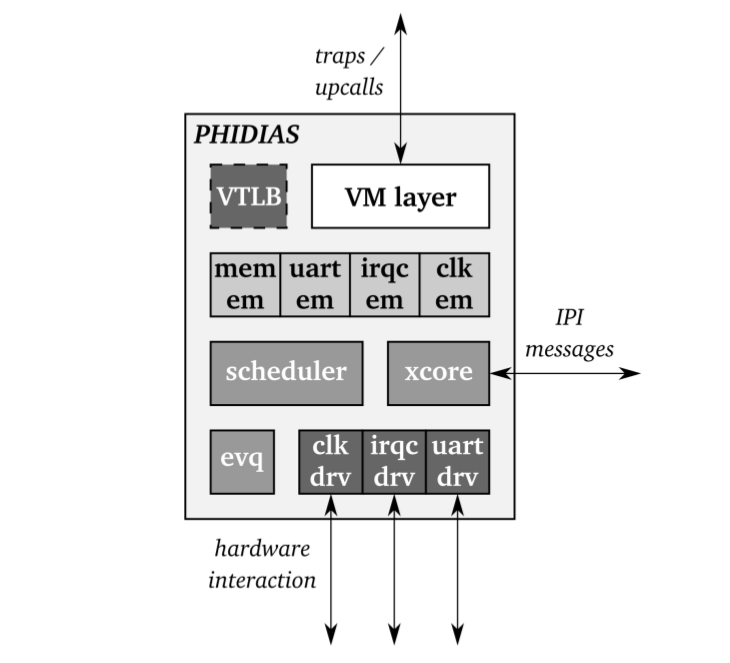
\includegraphics[width=10cm]{Phidias_Structure}
	\caption{Phidias Structure. Taken from \cite{Jan}}
	\label{Phidias_Structure}
\end{figure}

All mandatory components which are required for a hypervisor to function correctly are implemented in PHIDIAS. Following is a brief description of each of these basic components.\\
\\
\subsubsection{VM Layer}
VM Layer is responsible for performing world switch between guests and hypervisor. It performs upcall to enter into guests world and dispatches events to appropriate components for handling them. 
\subsubsection{Emulation Layer}
Emulation layer consists of minimal implementation of components necessary for hypervisor to operate. It includes UART, clock, Interrupt controller and a generic memory emulation. Generic memory emulation is added to run unmodified platform-specific Linux kernels without breaking their device specific functionality. Device driver sends memory requests to expected addresses but gets zero on reads and writes are discarded.
\subsubsection{Scheduler and Xcore}
At the heart of PHIDIAS, there is a scheduler with simple single-priority round-robin policy and Xcore components for relaying interprocessor interrupts between different instances of hypervisor and triggering interrupt capabilities.
\subsubsection{Event Queue and Drivers for emulation}
There is an event queue which is responsible for keeping track of programmed timer events and emulation drivers for minimal functionality is also present.

\subsection{Static Configuration and Final Image}
PHIDIAS is a static hypervisor which is built using a modifiable scenario specific configuration through an XML based compile time utility called Schism, the “Static Configurator for Hypervisor-Integrated Scenario
Metadata”. There are two types of configuration elements i.e. Hypervisor configuration and VM specific configuration elements.
\subsubsection{Hypervisor Configuration Elements}
\begin{itemize}
	\item Selection of CPU architecture and target platform SoC
	\item Physical and virtual Hypervisor base load address
	\item Selection of drivers for hardware devices and for the required emulation devices
\end{itemize}
\subsubsection{VM specific Configuration Elements}
\begin{itemize}
	\item Number of virtual CPUs per guest
	\item memory configuration per guest
	\item List of capabilities of each VM
	\item Assignments of pass-through interrupts to VMs
	\item Types, parameters, and corresponding emulated memory for selected emulated devices
\end{itemize}


    \chapter{Overview of Xen\label{cha:chapter3}}
This section provides background information on the Xen hypervisor and core components of its split device driver architecture for I/O emulation.

\section{Introduction of Xen\label{sec:xen}}
The Xen Project hypervisor is an open-source type-1 or baremetal hypervisor, which makes it possible to run many instances of an operating system or indeed different operating systems in parallel on a single machine (or host) \cite{xen}. It is one of the popular open-source hypervisors which can provide both para-virtualization and full virtualization solutions.In fact, it is the only available type-1 hypervisor which is open-source. It has been used in server and desktop virtualization and fueling the biggest clouds and web services in production today e.g. Amazon Web Services. 
\\
\\
Xen was developed at University of Cambridge in 2003 by Ian Pratt, a senior lecturer in the Computer Laboratory, and his PhD student Keir Fraser \cite{xen_wiki}. It was acquired by Citrix in 2007. Since April 15, 2013, Xen Project has become a Linux Foundation Collaborative Project with the following companies  contributing to and guiding the Xen Project as founding members are: Amazon Web Services, AMD, Bromium, Calxeda, CA Technologies, Cisco, Citrix, Google, Intel, Oracle, Samsung and Verizon \cite{xen_news}.
\\
\\
The basic components which work together to provide virtualization solution include Xen Hypervisor, Privileged guests called \textbf{Domain-0 or Dom0} and unprivileged guests called \textbf{Domain-U or DomU}. Xen hypervisor is a small software which directly runs on hardware and is responsible for CPU scheduling ,memory management and interrupt handling. After Xen hypervisor is booted, it launches Domain-0 guest which has direct access to all hardware and has native device drivers for performing I/O operations. Other unprivileged guests or domains access hardware and perform I/O via Dom0. Dom0 is also responsible for launching and managing DomUs with the help of control stack called Toolstack running on it. Figure \ref{xen_arch} shows the architecture of Xen virtual environment.
\begin{figure}[!htbp]
	\centering
	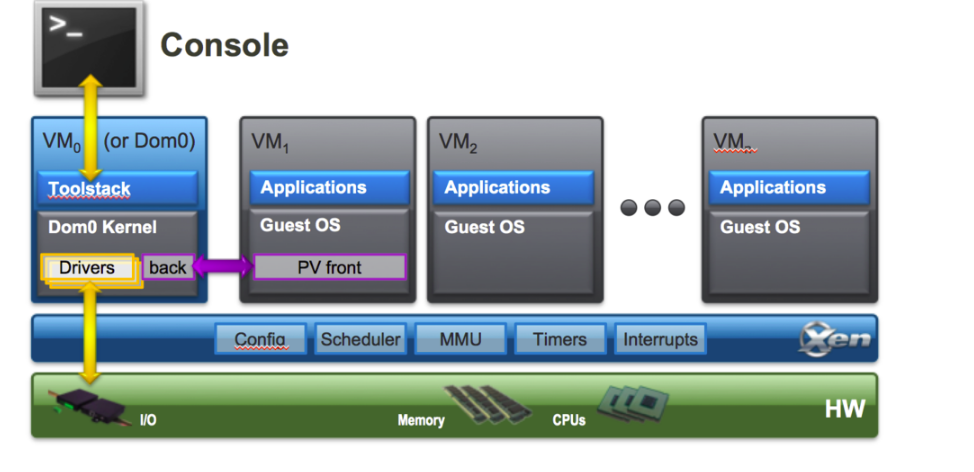
\includegraphics[width=10cm]{xen_arch}
	\caption{Xen Architecture Taken from \cite{xen_wiki}}
	\label{xen_arch}
\end{figure}
\\
\\
\subsection{Guest Virtualization Types in Xen \label{sec:guests}}
Xen provides two types of virtualization modes for guests:
\begin{itemize}
	\item  \textbf{Paravirtualization (PV)}, first introduced by Xen, is virtualization technique in which guests are modified and are aware of being run on a hypervisor. A PV guest requires PV enabled kernel and PV drivers to be present to run without emulation. Dom0 in Xen is a privileged PV guest which has access to actual device drivers and hardware in the system and provides an interface to control and manage other VMs.
	\item \textbf{ Hardware-assisted or Full Virtualization (HVM)} is a virtualization mode which requires virtualization hardware extensions (Intel VT or AMD-V hardware extensions) to be present on host CPU. Guests kernels are used unmodified and hence Windows can run as HVM guest on Xen.Xen uses Qemu on HVM guests for hardware emulation and hence are slower than PV guests. However, paravirtualized drivers can be used for I/O on HVM guests to increase performance of system.
\end{itemize}

Guests with both types of virtualization can be run at the same time on Xen. It is also possible to use paravirtualization on HVM guests and vice versa. This mixing of modes has introduced two more modes of virtualization on Xen which are PVHVM and PVH. In PVHVM guests, optimized paravirtualized drivers are used for disk and network virtualization on hosts with hardware virtualization extensions enabled. PVH are basically paravirtualized guests which use PV drivers for I/O operations and use hardware virtualization extensions for others.
\\
\\
There are pros and cons of each mode of virtualization in Xen. Full virtualization provides full emulation of underlying hardware to guests which require no modifications in their OSes. However, performance is degraded while providing full emulation of entire system by VMM. Also HVM guests use trap and emulate model for execution of sensitive and privileged instructions which can cost to hundreds to thousands of cycles \cite{wang2010dynamic}.. On the other hand, paravirtualization allows modified guests to run on a system with an abstraction of similar physical hardware on system and hence provides near native performance as compared to HVM guests. It replaces the sensitive instructions with hypercalls to VMM and allows combining several hypercalls into one hypercall to reduce transitions between Guests OS and VMM \cite{wang2010dynamic}.

\section{Device I/O Emulation on Xen\label{sec:xendevice}}
Xen hypervisor virtualizes CPU, memory, interrupts and timer. It does not have any knowledge of I/O devices. Access to actual physical I/O devices and their native device drivers is present in privileged Domain-0. Unprivileged guests can get access to I/O devices through Dom0. Xen assigns all I/O devices to Dom0 which is then responsible for MMIO remapping and interrupt handling. \\
\\
Device virtualization in Xen is done using a pair of paravirtualized drivers called \textbf{frontend and backend drivers}. For each class of hardware devices i.e. disk, network, console, framebuffer, mouse, keyboard, etc, a pair of paravirtualized drivers is present in system. Paravirtualized backends are implemented in Dom0 with their corresponding frontends being implemented in DomU. These paravirtualized drivers are implemented as kernel drivers. However, some backends can run in QEMU in userspace. Communication between frontends and backends is done through a shared memory ring protocol and events notifications mechanism provided by Xen. Xen provides tools to setup communication framework between frontend and backend drivers in Dom0 \cite{xen_arm}. Figure \ref{xen_device} shows the I/O device virtualization architecture in Xen.

\begin{figure}[!htbp]
	\centering
	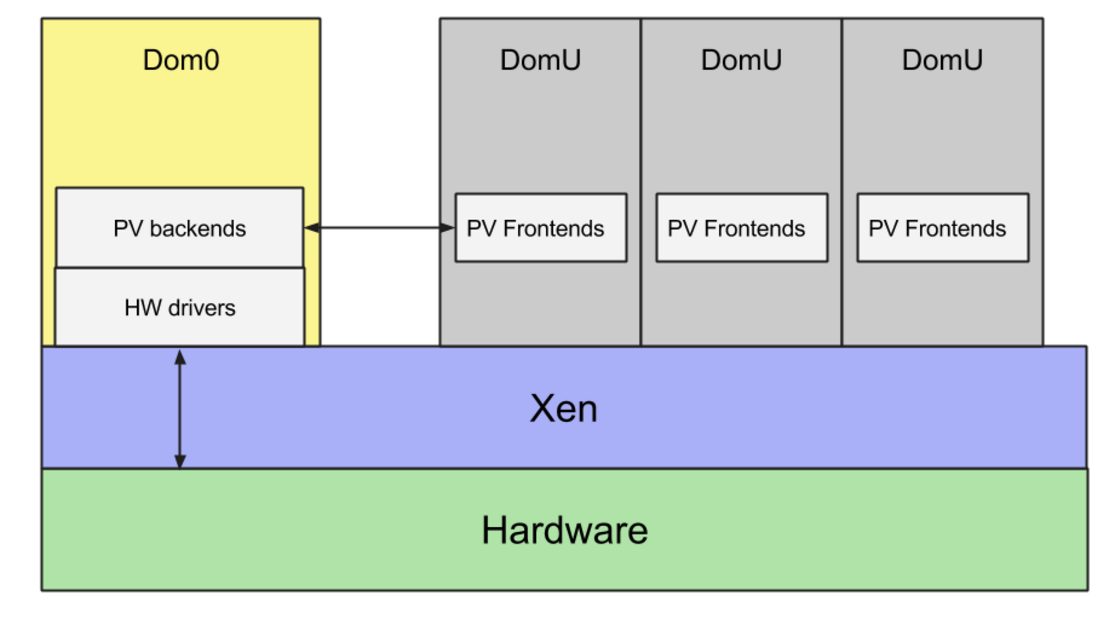
\includegraphics[width=10cm]{XEN_Device_Arch}
	\caption{Xen I/O Device Virtualization Architecture. Taken from \cite{xen_arm}}
	\label{XEN_Device_Arch}
\end{figure}

In order to provide isolation, security and disaggregation, Xen has introduced the concept of driver domains. Such domains are unprivileged guests running backends and native drivers for I/O device virtualization. If such a domain is compromised or crashed, it will not affect other guests or domains. Figure \ref{driver_domain} shows the architecture of driver domains in Xen.

\begin{figure}[!htbp]
	\centering
	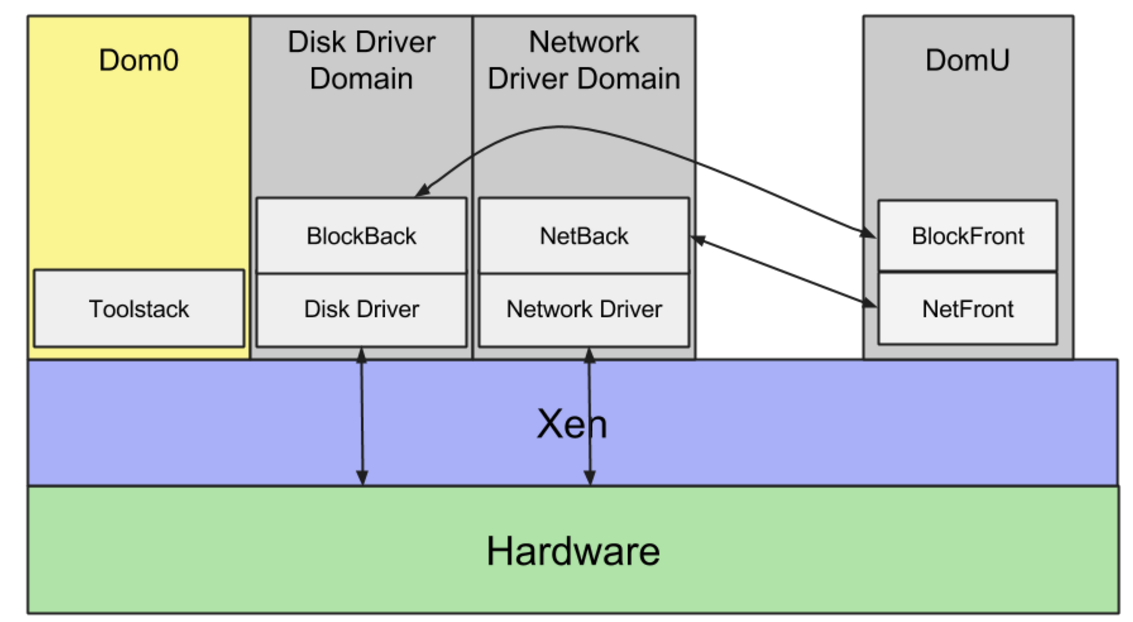
\includegraphics[width=10cm]{driver_domain}
	\caption{Xen Driver Domains Architecture. Taken from  \cite{xen_arm}}
	\label{driver_domain}
\end{figure}

\subsection{Xen on ARM\label{sec:xendevice}}
Xen on ARM is a simple, smaller and faster as compared to its x86 counterpart. The main features of Xen on ARM are described as follows:
\begin{itemize}
	\item It does not perform any emulation. There is no QEMU emulation in Xen on ARM.
	\item It exploits hardware virtualization support for memory management, interrupts and timer virtualization.
	\item It uses paravirtualized pair of drivers for I/O virtualization.
	\item It runs entirely in hypervisor mode and provides an HVV hypercall to kernels to switch between hypervisor mode and kernel mode.
	\item It uses virtualization aware Generic Interrupt Controller for interrupt handling.
	\item It uses virtualization aware Generic Timers to provide timer virtualization to guests.
	\item It supports one type of guests which exploits hardware virtualization as much as possible and uses paravirtualized interfaces for I/O device virtualization.
\end{itemize}

Figure \ref{xen_on_arm} shows the simple architecture for Xen on ARM platforms.
\begin{figure}[!htbp]
	\centering
	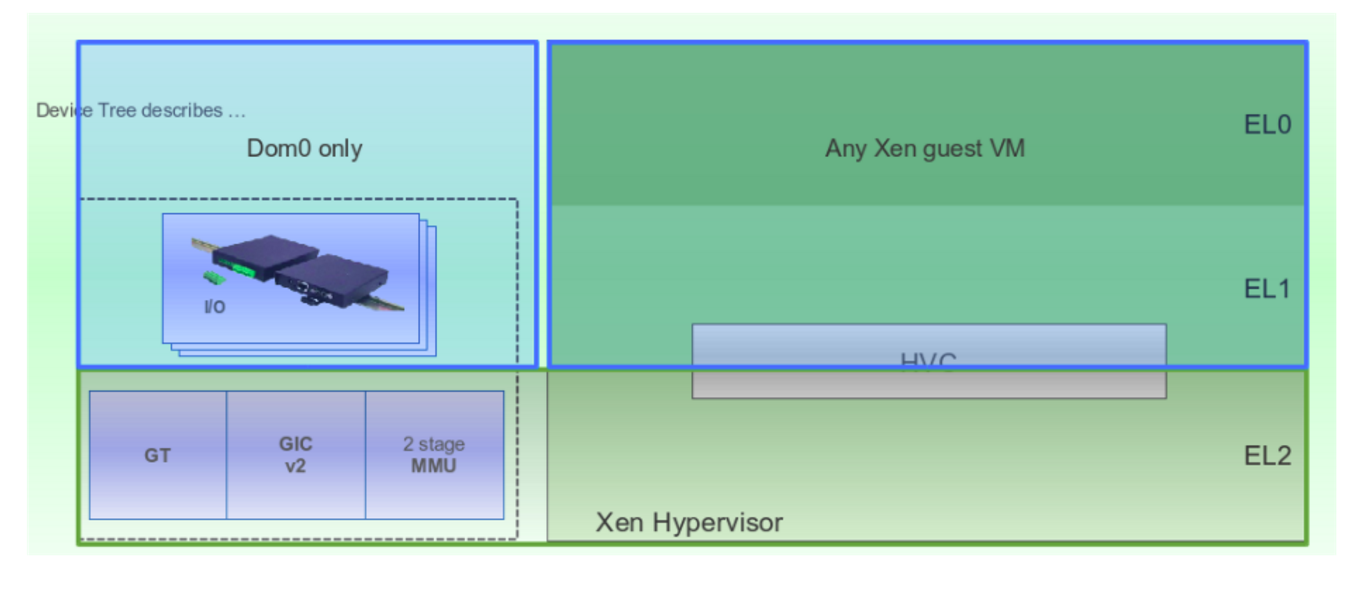
\includegraphics[width=10cm]{xen_on_arm}
	\caption{Xen on ARM Architecture. Taken from  \cite{xen_arm}}
	\label{xen_on_arm}
\end{figure}

\section{Xen Split I/O Driver Model\label{sec:xensplit}}
With the widespread use of embedded systems in multiple applications, diversity in I/O devices used by such systems has increased significantly. Supporting a large of I/O devices in Xen would make things worse for maintaining Xen hypervisor code and avoiding bugs. Most operating systems e.g Linux provide support for a large number of devices and reusing this capability would make a cleaner, smaller and much simpler hypervisor. Xen has delegated all I/O hardware devices to privileged Domain-0 or special unprivileged driver domains. All other guests access I/O devices through Dom0 or driver domains. Xen provides mechanisms for communication between guests which use split driver model for multiplexing and using hardware I/O devices. Xen support Net, Block, console, keyboard, mouse, framebuffer, XenGT(intel Graphic
card), 9pfs, PVCalls, Multi Touch, Sound and Display devices \cite{xen_release}. In the next sections, details of basic components of split driver model of Xen will be explained.

\subsection{Basic Components of Xen Split I/O Driver Model\label{sec:basiccomp}}
Xen device drivers typically consists of four major components:
\begin{itemize}
	\item The native I/O device driver
	\item Top half or Frontend of the split driver
	\item Bottom half or backend of the split driver
	\item Shared ring buffers
\end{itemize}

The real drivers for I/O devices are present in Dom0 or driver domains for accessing actual hardware. They are interfaced with backend drivers of the split driver which provides a generic interface and I/O device multiplexing functionality. Frontend driver is present in unprivileged guests and communicate with backends using shared memory ring buffers. Frontends write requests on these buffers and backends write responses which are signaled through xen event notification mechanism. Successful shared memory communication between frontend and backend requires xen grant tables, event channels, xen bus and Xenstore to be working in system. These mechanism will be explained in the later sections. Figure \ref{splitdevice} shows the basic architecture of Xen split driver mode.
\begin{figure}[!htbp]
	\centering
	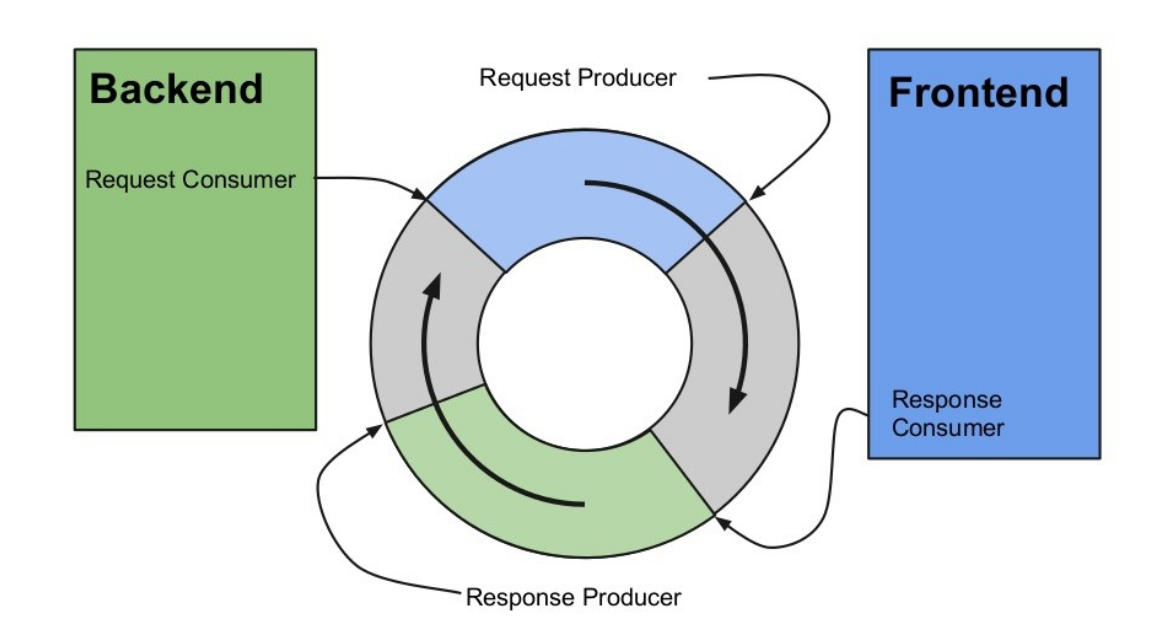
\includegraphics[width=10cm]{splitdevice}
	\caption{Basic Xen Split Driver Architecture. Taken from \cite{xen_slides}}
	\label{splitdevice}
\end{figure}

\subsection{Xen mechansims used by Split I/O Driver Model\label{sec:basicmech}}
There are basically four mechanisms provided by Xen which are used by Split Driver model of Xen to work successfully. These are as follows:
\begin{itemize}
	\item Grant Tables
	\item Event Channels
    \item Xenstore
	\item XenBus Protocol
\end{itemize}
The split drivers across domains use these mechanisms to communicate and access hardware devices. Following sections provide brief explanation of each of these mechanisms.
\subsubsection{Xen Grant Tables\label{sec:granttables}}
Grant tables is a mechanism to provide shared memory to guests. Each guests can manipulate the shared memory on page level granularity. Grant tables provides two types of memory sharing operations to guests i.e. memory sharing and memory transferring. Since all physical memory is mapped by Xen hypervisor, copying the data between domains is done by hypervisor without modifying page tables. Transferring a page from one domain to another is also available which changes the page owner and modifies the page tables accordingly. To identify the page being shared or transferred, guests uses grant references which are integers indexed into an array of grant entries in grant table. These grant references are placed in Xenstore ,a virtual file system for device discovery in Xen, to communicate shared page information to other domains.
\\
\\
The interface to grant tables is provides by Xen in the form of hypercalls for grant table operations. Two basic operations that can be performed on grant tables are mapping and transferring pages. Mapping a page removes original reference of page in sender domain's address space while transferring causes the page to leave calling domain's address space. Mapping is used by drivers to implement interdomain communication using shared memory while transferring is used to move data between domains. 
\\
\\
Xen hypervisor creates four types of structures to implement grant table mechanism:
\begin{itemize}
	\item Shared Grant table is created and shared by Xen for each guest. Guest writes into entries in table and Xen performs the desired operation specified by hypercalls. Four pages are allocated and shared with each guest during initialization of each domain. A maximum of 32 pages can be allocated for shared grant tables.
	\item Active Grant table is created and maintained by Xen to keep track of active grants per domain. Four pages are allocated initially for implementing active grant table per domain by Xen.
	\item Mapped track table is created and maintained by Xen per domain for each mapped page. Initially 1024 map track entries are allocated for each domain by Xen.
	\item Status Grant table is created and maintained by Xen for keeping track of status of each grant per domain.
\end{itemize}
Figure \ref{granttable} shows the basic structure of shared grant table.

\begin{figure}[!htbp]
	\centering
	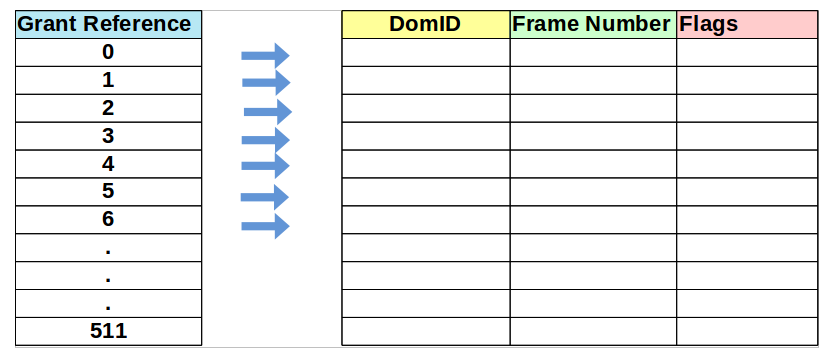
\includegraphics[width=10cm]{granttable}
	\caption{Basic structure of shared Grant table}
	\label{granttable}
\end{figure}
\textbf{Grant Table Use for Shared Ring Buffers}
Device I/O rings which are used for communication between split drivers are built on top of shared memory provided by grant table mechanism. Frontend drivers creates ring buffer pages and grant access to backend. Backend drivers map these shared pages for ring buffers and communication channel is established across domains. Figure \ref{ring} shows the actions performed by split drivers on ring buffers for interdomain communication.

\begin{figure}[!htbp]
	\centering
	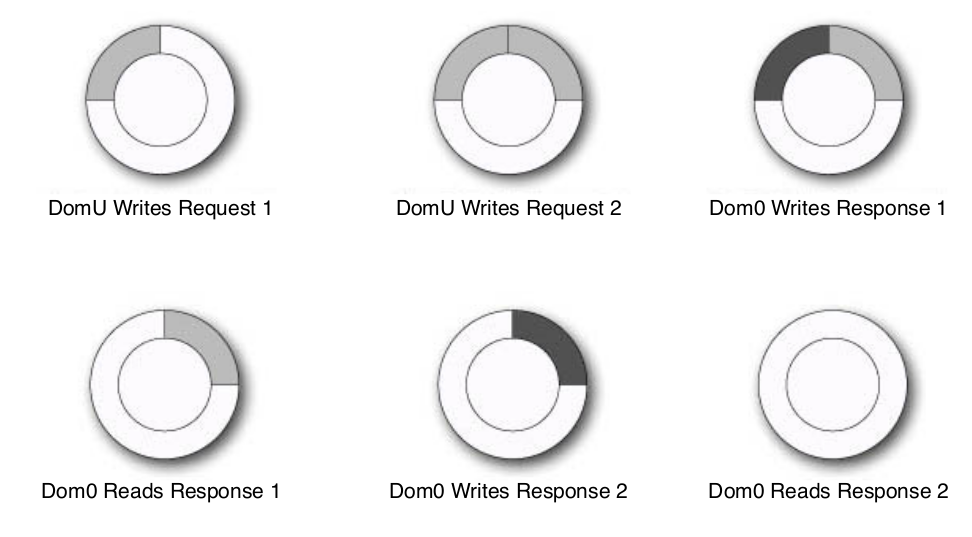
\includegraphics[width=10cm]{ring}
	\caption{Request/Response sequence on ring buffers. Taken from \cite{xen_book}}
	\label{ring}
\end{figure}
\subsubsection{Xen Event Channels\label{sec:eventchannel}}
Event channels is a mechanism for asynchronous delivery of notifications between domains. These are used with shared memory mechanism to provide message passing between split drivers in domains. Events are similar to Unix signals. Each event represents one bit of information about which event has occured. There are four types of event channels supported by Xen:
\begin{itemize}
	\item Interdomain events are used by split drivers for notifying each other about data waiting to be transported to other domain.  These are bi-directional.
	\item Physical IRQ are used to bind actual hardware IRQs to event channels. These are used by Domain-0 or driver domains to access various devices under their control by mapping physical IRQs to event channels.
	\item virtual IRQs (VIRQ) are used to bind IRQs of virtual devices e.g virtual timer or emergency console to event channels.
	\item Intradomain events are used to send events between virtual CPUs of a single domain similar to interprocessor interrupt (IPI) mechanism. These are bi-directional.
\end{itemize}

Event channel creation is a two-stage process. In the first step, an event source is bound to event channel and in second step, an event handler is registered for handling triggered event. Event channel is an abstraction of sending asynchronous notifications between domains. Each channel has two endpoints which are called ports in local domain. After binding an event channel to remote port, a domain can send an event to local port via hypercall through Xen hypervisor. Xen is then responsible for finding the remote end of channel and remote domain and route events to destination.
\\
\\
Each virtual CPU in the guest on Xen has an event channel bitmap associated with it. This event channel bitmap is shared with Xen in shared info page created during initialization of guest. When an event is received by Xen for a particular guest, it sets event channel upcall pending flag, desired bit of event and corresponding word which contains set event bit. All these fields are present in shared info page. There are also mask bits for disabling event delivery to guests. Events delivery can be masked both by individual event type or disabling/enabling all together.
\\
\\
Two implementations of event channels are supported in Xen \cite{xen_events}:
\begin{itemize}
	\item 2-level event channel ABI is de-factor implementation for event channel mechanism for which 32 bit domain supports up to 1024 event channels and 64 bit domain supports up to 4096 channels.A 2-level search path is used for finding the set event bit in event channel bitmap. For the thesis, 2-level event channel has used since it meets the requirements for porting I/O split driver to PHIDIAS.
	\item FIFO-based event channel ABI has lockless queues for event queues with configurable number of event channels and event priorities. It can support more thanm 100,000 event channels, with scope for  16 different event priorities.
\end{itemize}
Figure \ref{events_slide} shows the basic architecture of 2-level event channel implementation.

\begin{figure}[!htbp]
	\centering
	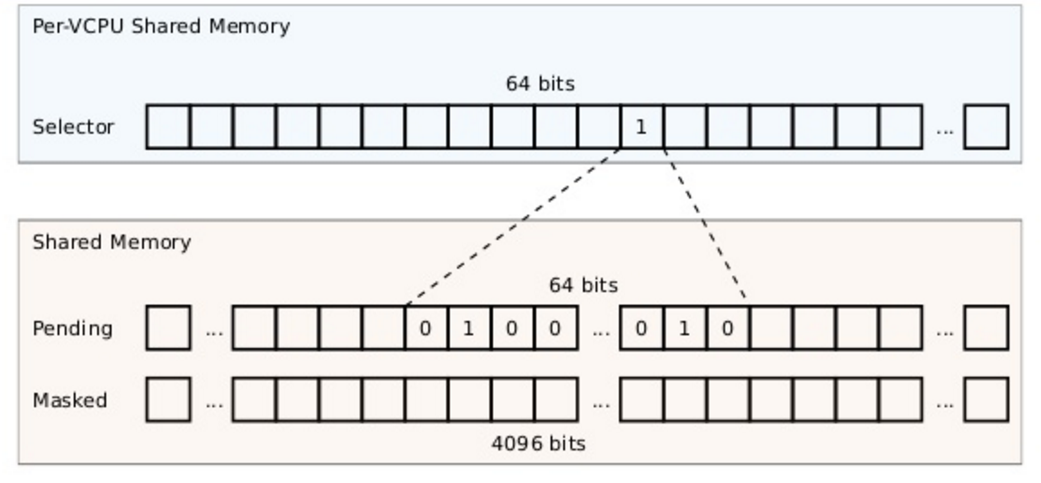
\includegraphics[width=10cm]{events_slide}
	\caption{2-level event channel implementation in Xen. Taken from \cite{events_slide}}
	\label{events_slide}
\end{figure}
\subsubsection{Xenstore \label{sec:xenstore}}


    \chapter{Porting Environment and Requirements\label{cha:chapter4}}
In this chapter, the basic requirements and environmental setup for porting Xen split driver model to PHIDIAS will be discussed. 

\section{Environmental Setup for Porting\label{sec:xen}}
Basic environment for this thesis consisted of an ARM target platform and a Linux PC with required tools and source code. The details of target platform and source code used are given below.

\subsection{Target Platform\label{sec:xen}}
HiKey (LeMaker version) \cite{hikey} was used as a target platform which has the following features:
\begin{itemize}
	\item Kirin 620 SoC
	\item ARM Cortex-A53 Octa-core 64-bit up to 1.2GHz (ARM v8 instruction set)
	\item 2GB LPDDR3 DRAM
	\item On-board 8GB eMMC nand flash storage
	\item TI WL1835MOD 2.4 GHz Wireless card
\end{itemize}

\subsection{Linux kernel version\label{sec:xen}}
The Linux kernel used for running Xen on HiKey was 4.1.15 obtained from \cite{96boards_2016}. Linux kernel used for running PHIDIAS was linux-4.11-rc2 obtained from \cite{linux4_11}. 

\subsection{Xen version\label{sec:xen}}
Xen 4.7.0 was used for setting up reference framework for porting taken from \cite{xengit}.

\subsection{PHIDIAS version\label{sec:xen}}
Table \ref{PHIDIAS_comp} describes commit ids for components of PHIDIAS and their git repositories used in current project.

\begin{table}[!htbp]
	\centering
	\begin{tabular}[t]{|C{3cm}|C{4cm}  |C{4cm}|}
		\hline
		PHIDIAS component & commit id & git repo \\
		\hline
		xml &  30d880a5b2b28c7032c & git@gitlab.sec.t-labs.tu-berlin.de:phidias\\
		& dce4b564496ab08f06a15 &/xml.git \\
		\hline
		core & 3a1771b3aa6cf2b789805 & git@gitlab.sec.t-labs.tu-berlin.de:phidias\\
		& d849e74e8ffbdc9dbc3 & /serial\_multiplexer.git \\
		\hline
		abi &  8d8c3d1251799701eb& git@gitlab.sec.t-labs.tu-berlin.de:phidias/abi.git\\
		& 82e5a54fb7ec8075a30ce & \\
		\hline
		serial\_multiplexer & 968b913fa865e7129a9 & git@gitlab.sec.t-labs.tu-berlin.de:phidias \\
		& 10c79818153b361cbaf6e & /serial\_multiplexer.git\\
		\hline
	\end{tabular}
	\caption{Description of PHIDIAS components commit ids and git repos used for porting}
	\label{PHIDIAS_comp}
\end{table}

\section{Requirements for Porting\label{sec:xen}}
Following requirements were considered and fulfilled while porting Xen I/O split driver model to PHIDIAS:
\begin{itemize}
	\item Keep the changes as minimum as possible in PHIDIAS hypervisor code. For the current project, no additional changes are added in PHIDIAS besides adding serial multiplexer functionality for getting serial output from guests running on different physical CPUs.
	\item Keep the changes as minimum as possible in Xen domains Linux source code and make changes in separate generic interfaces exposed to all xen's split drivers. This also has been satisfied in current work by adding changes usable by split drivers for all types of I/O devices.
	\item Add required changes in Linux kernel code cleanly easy to maintain future releases. Two major changes were added for porting work. One was to create a separate memory ZONE name ZONE\_XEN in Linux kernel used by split drivers for allocating pages for sharing and another was to register a custom IPI handler for software generated interrupts.
	\item Port Xen's frontend and backend of network virtual device to PHIDIAS for the proof of concept of flexibility of the static hypervisor and adding networking support between guests.
	\item Tools (iperf and ping) which are used for testing should be same. Ping utility used is of BusyBox v1.22.1 and iperf is of version 2.0.10 (11 Aug 2017) pthreads.
	\item Keep changes small in Xenstore userspace tool. For current work, only one change is added to introduce domU with Xenstore manually. In original Xen setup, this is done via XL tool as explained previously \ref{sec:xenstore}  which depends upon Xen hypervisor hence not used in our porting setup.
	\item At least two guests should be able to communicate via ported split driver.
\end{itemize}


    \chapter{Design and Implementation: Porting Xen Split Driver Model to PHIDIAS\label{cha:chapter5}}
For porting Xen split driver model, three major components i.e. Grant tables, Event channels and Xenstore are modified to use static memory and PHIDIAS's xcore and capability feature. In this chapter, I will explain how PHIDIAS's \textit{\textbf{Principle of Staticity}} could be applied to to Xen I/O drivers.

\section{Porting Xen I/O Virtualization Framework to PHIDIAS\label{sec:memstatic}}
All necessary porting done in core components of Xen I/O virtualization framework will be discussed in this section.

\subsection{Porting of Shared Information Pages\label{sec:sharedinfo}}
Shared info page is used to share virtual machine state with Xen hypervisor. It includes information about virtual CPU (vCPU) state, event channels and wall clock time information. Each guest allocates a zeroed page for shared info page from kernel and registers it with Xen hypervisor through a hypercall. In our case, a static memory range has been configured to allocate shared info pages. These pages are shared between guests instead with the PHIDIAS hypervisor. Size of this static memory range is configurable and depends upon the total number of configured guests in system. Each guest obtains its share info page from this static contiguous memory range using its domain ID config option \textbf{CONFIG\_XEN\_DOM\_ID} as shown in listing \ref{sharedpage}. \\
\\
\begin{lstlisting}[caption=Guest mapping its shared information page on PHIDIAS, label={sharedpage}]
Shared_info_pages = (unsigned long)xen_remap(0xfee43000, XEN_PAGE_SIZE * 2);
if (!Shared_info_pages) {
pr_err("not enough memory\n");
return -ENOMEM;
}

if (xen_initial_domain())
memset_io((void *)Shared_info_pages, 0, XEN_PAGE_SIZE * 2);	

HYPERVISOR_shared_info = (struct shared_info *)(Shared_info_pages + (XEN_PAGE_SIZE * CONFIG_XEN_DOM_ID));
\end{lstlisting}
Dom0 with ID 0 initializes the entire range with zeros. The shared info page is mapped in linux guest as un-cached so that other guests would get the consistent view of each other's shared information. Figure \ref{sharedinfo} shows the approach of implementing shared info pages for two guests in PHIDIAS.
\\


\begin{figure}[!htbp]
	\centering
	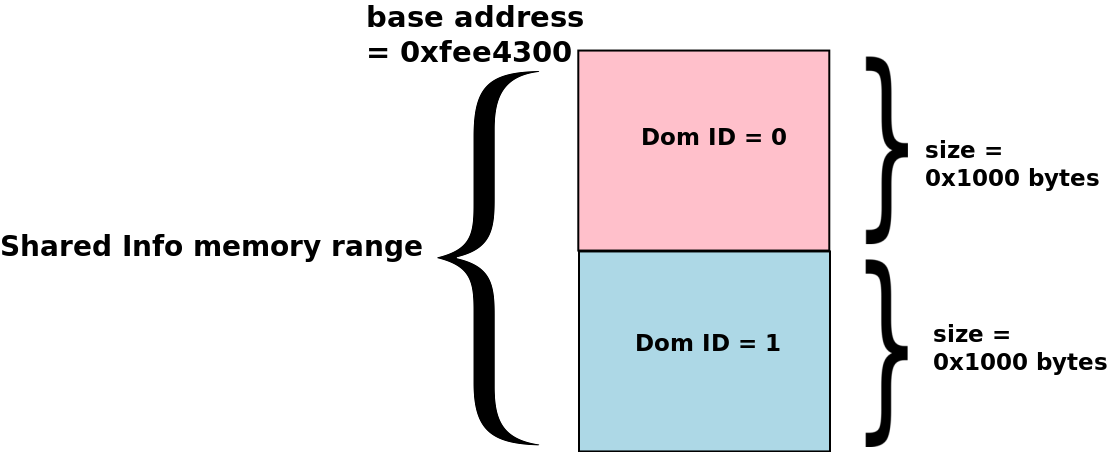
\includegraphics[width=10cm]{sharedinfo}
	\caption{Basic approach of implementation of shared info pages in PHIDIAS for two guests}
	\label{sharedinfo}
\end{figure}


\section{Porting of Grant Tables\label{sec:granttablesstatic}}
As described in \ref{sec:granttables}, grant tables are a mechanism for sharing memory pages across domains. Xen hypervisor allocates pages for grant tables per domain and guests map them into their address spaces. By design, Xen does not support swapping which means that even unused part from the allocated memory of a guest could not be used by other guests. To solve this problem, Xen uses \textbf{ballooning}. Ballooning is way of dynamically increasing or decreasing size of allocated memory. Memory visible to each guest can be configured in Xen at boot time. For Dom0, it could be specified in grub configuration file and for domU, it is specified in XL tool's guest configuration file. If the guest uses less memory than configured amount, it can return unused blocks of memory to hypervisor. However, guest can not retrieve more memory from hypervisor's memory pool through ballooning than its maximum configured amount specified during its startup. Memory allocated to unprivileged guests is taken from Dom0 memory pool and hence Dom0 memory balloon's down every time a new guest is started.
\\
\\
For the current work, Xen balloon driver has been disabled in Linux guest kernel using configuration option CONFIG\_XEN\_BALLOON. In the native code of Xen's PV split drivers, ballooning is used to allocate pages for grant tables, XenBus ring buffers and mapping received network packets in network backend driver from the related frontend. In our ported setup, it has been replaced by defining two static globally shared readable/writable memory ranges for PHIDIAS's guests. One memory range is defined to allocate static memory for grant table frames while the other is defined to be used by all split drivers for establishing communication for I/O virtualization. Guests allocates required pages from these two memory ranges and map them un-cached into their respective address spaces. These two memory ranges will be explained in more detail in the following sections.

\subsection{Static Memory for Grant Frames\label{sec:granttablesframes}}
In Xen, maximum number of grant frames is defined to be 32. For the current thesis, since two guests were used for testing, a total of 64 contiguous pages had been configured for grant tables usage. Each guest had used 32 pages for its own grant table implementation. In our setup, every guest had access to other guests' grant table through un-cached mapping of their grant pages into its address space. For performing grant table operations, I/O split drivers of Xen find a reference or index of unused entry in their guest's grant tables and update this entry with fields of corresponding domain ID, shared frame number and desired flags. The guest then sends the obtained grant reference through ring buffers to the other guest. In native Xen setup, hypercalls are used to perform grant operations i.e. granting access to remote domain, mapping, transferring and copying pages across domains. In our ported setup, since each guest had access to remote's dguest's grant tables by mapping them directly into its address space, a local guest could perform direct operations by manipulating the fields in grant table entries of a remote guest. Listing \ref{grantmap} shows how a guest mapped remote guest's grant table into its domain in our setup. Figure \ref{grant_table} shows the configuration of grant table static memory range for two guests in PHIDIAS.
\begin{figure}[!htbp]
	\centering
	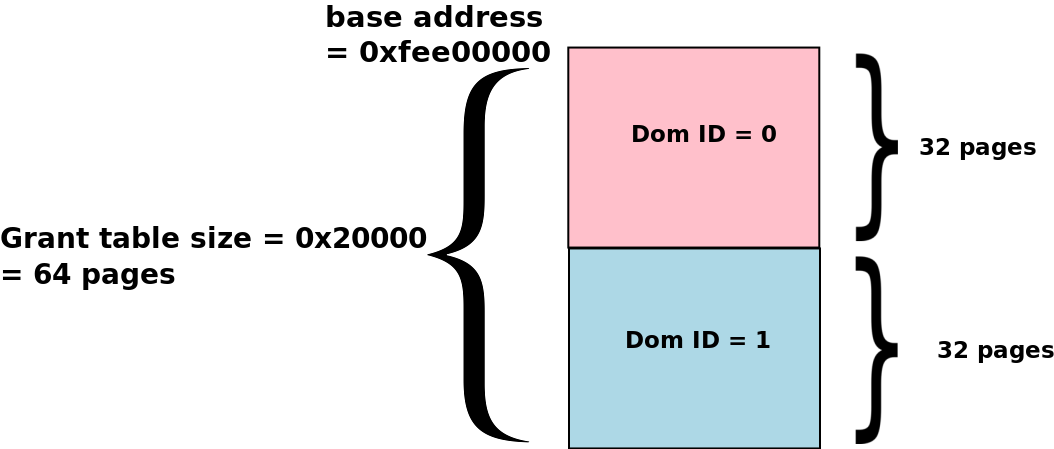
\includegraphics[width=10cm]{grant_table}
	\caption{Static memory configuration for grant table in PHIDIAS for two guests}
	\label{grant_table}
\end{figure}
\begin{lstlisting}[caption=Code snippet for mapping remote guest's grant table in case of two guests configured for the ported setup , label={grantmap}]
static int gnttab_setup(void)
{ ...
        gnttab_shared.addr = xen_auto_xlat_grant_frames.vaddr;
        
        if(xen_initial_domain())
            remote_grant_frames = 0xfee00000 + (0x20000 * 1) ;
        else
            remote_grant_frames = 0xfee00000 + (0x20000 * 0) ;
            
        vaddr = xen_remap(remote_grant_frames, XEN_PAGE_SIZE * max_nr_gframes);
        
        gnttab_shared_remote.addr = vaddr;
...
}
\end{lstlisting}

\subsection{Static Memory for I/O Split Drivers Usage\label{sec:splitdriverusage}}
I/O Split drivers of Xen guests play with memory using a set of in-built kernel functions e.g alloc\_page, free\_page etc. However, they share those pages with other guests through Xen's grant table hypercalls. In order to use the same Linux page allocation APIs and keep changes in split drivers as minimum as possible, a new memory zone named \textbf{ZONE\_XEN} had been added in Linux kernel for our setup. A static globally- shared memory range of size 8192 KB has been configured in PHIDIAS for two guests. Size of ZONE\_XEN for each guest was set to 4096 KB i.e. 1024 pages. Each guest obtained the starting address of its zone using the base address of configured shared memory range of size 8192 KB and its domain ID as shown in listing  \ref{list_zone}.
\\
\begin{lstlisting}[caption=Code snippet for calculating start address of guest ZONE\_XEN, label={list_zone}]
    xen_zone_size = 0x400000;
    xen_zone_start_addr = 0xfef00000 + (CONFIG_XEN_DOM_ID * xen_zone_size);

\end{lstlisting}
Figure \ref{zone_xen} shows the memory configuration for areas of ZONE\_XEN for two guests in PHIDIAS.
\begin{figure}[!htbp]
	\centering
	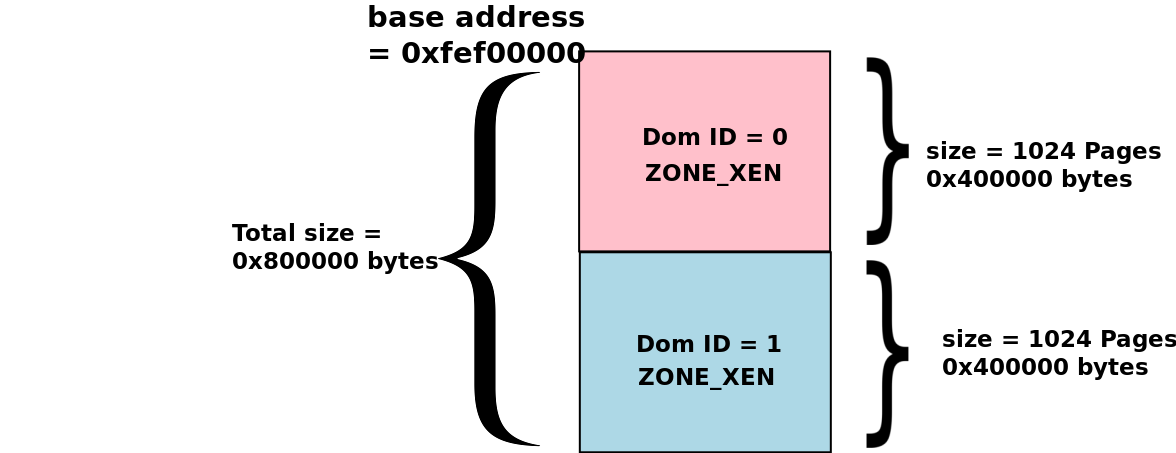
\includegraphics[width=10cm]{zone_xen}
	\caption{Static memory configuration for ZONE\_XEN in PHIDIAS for two guests}
	\label{zone_xen}
\end{figure}
Since the entire zone memory range is shared between two guests in our setup, each guest could easily calculate the starting address of other guest's zone space. In order to access pages granted for sharing by a remote's guest, the local guest should map those pages into its address space so that it could read or write on those shared pages. In native Xen setup, Xen hypervisor is responsible for modifying page tables and sharing of pages across domains. However, in our setup, we have to map all pages of other's guest ZONE\_XEN into local guest address space before accessing them through I/O split drivers. We cannot use \textbf{ioremap} function when grant operations are called by split I/O driver e.g in \_\_gnttab\_map\_grant\_ref and gnttab\_batch\_copy. The reason is that ioremap cannot be called in interrupt context and PV split drivers perform grant operations in this particular context. In order to solve this problem, whole zone area of other guest had been mapped in local guest's address space during initialization in arch\_gnttab\_init function as shown in listing \ref{hash}.\\
\\
\begin{lstlisting}[caption=Code snippet for populating hash table for virtual address mapping of shared pages for two guests in ported setup, label={hash}]
int arch_gnttab_init(unsigned long nr_shared)
{ ...

#if CONFIG_XEN_DOM_ID == 1
base_value = 1044224;
phys_addr = 0xfef00000;

#elif CONFIG_XEN_DOM_ID == 0
base_value = 1045248;
phys_addr = 0xFF300000;
#endif


virt_addr =  xen_remap( phys_addr , 0x400000);
for (i = 0; i< SIZE_ARRAY; i++)
{
key = phys_addr >> XEN_PAGE_SHIFT; 
hash_insert(key, virt_addr);
virt_addr = (unsigned long)(virt_addr) + 4096;
phys_addr = phys_addr + 4096;
}
..
}
\end{lstlisting}
Then a hash table had been created containing virtual addresses of these mapped pages indexed with their respective physical page frame numbers. This hash table had thus solved the following two problems:

\begin{itemize}
	\item Speed up the process of finding virtual address of remote's guest shared page by not mapping each page individually in grant table functions.
	\item Avoiding the use of ioremap in grant table functions since it cannot be called in interrupt context.
\end{itemize}

Figure \ref{hash_table} shows the basic structure of implemented hash table.

\begin{figure}[!htbp]
	\centering
	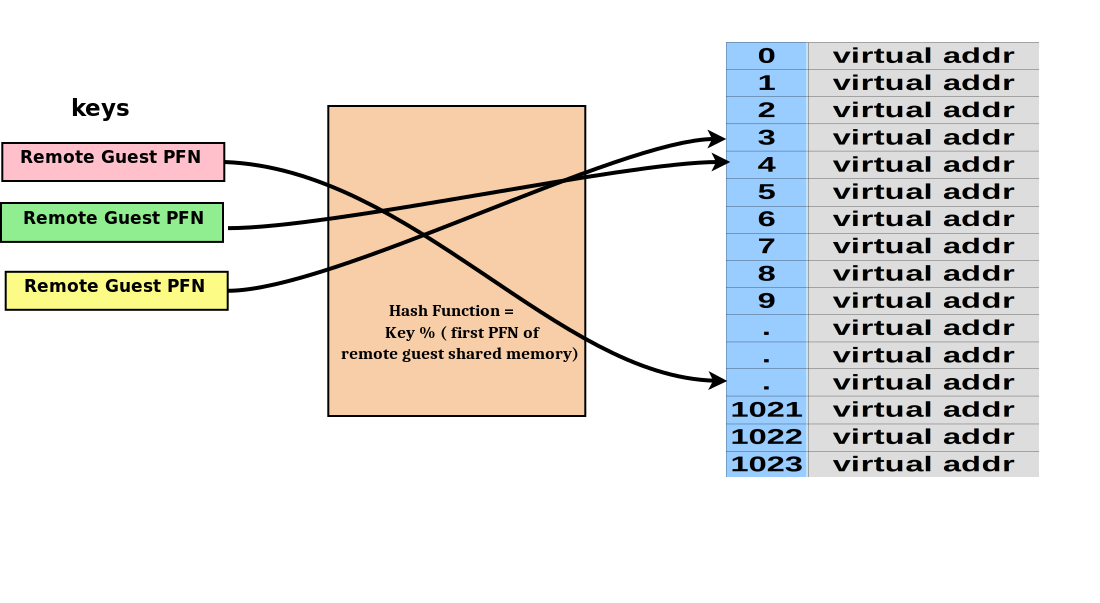
\includegraphics[width=10cm]{hash_table}
	\caption{Structure of hash table used for accessing remote guest's of ZONE\_XEN shared pages}
	\label{hash_table}
\end{figure}


\section{Design of Porting Event Channels\label{sec:eventstatic}}
As explained in section \ref{sec:eventchannel}, event channels are used to send asynchronous notifications among guests in Xen. On ARM, software generate interrupts (SGI) can be used for interprocessor communication. There are 16 SGI available on ARM architecture. For Xen guests, there is a common interrupt handler \textbf{xen\_arm\_callback} for handling notifications from remote guests via event channels. Xen guest uses PPI 31 for event IRQ which is configured in hypervisor node of its flattened device tree provided to it by Xen during its booting sequence as shown in listing \ref{xen_node}.
\\
\\
\begin{lstlisting}[caption=Xen Hypervisor node in hi6220 flattened device tree, label={xen_node}]
 hypervisor {
     compatible = "xen,xen", "xen,xen-4.7"; //version of the Xen ABI 
     reg = <0xb0000000 0x20000>;            // Grant table memory area 
     interrupts = <1 15 0xf08>;             //event notifications IRQ
 };

\end{lstlisting}
In PHIDIAS, SGIs have been used for implementing interprocessor interrupts using its \textbf{Xcore mechanism}. By default, first 6 SGI interrupts are used by Linux kernel. In our ported setup, we could use one of the remaining SGIs for registering \textbf{xen\_arm\_callback} handler for Xen event IRQ. However, in Linux kernel version 4.11\_rc2 used in this work, Linux kernel handle\_IPI function only processes first 6 SGIs. For remaining SGIs, it shows a default warning of \textit{Unknown IP}. To handle this, some modifications were made in IPI handling code of Linux kernel. For SGIs other than the default first six, modified IPI handling function is implemented for our setup. It checked whether some handler is registered for given interrupt number and then called respective handler if found any. An online resource \cite{smp} has been used as a reference for implementing this IPI handling function.
\\
\\
I had used SGI number 9 for triggering Xen events in PHIDIAS for inter-domain communication. 2-level event channel support had been ported which used two-level bitmap to speed searching. The first level is a bitset of words which contain pending event bits.  The second level is a bitset of pending events themselves. All event channel hypercalls in Xen guests were replaced with PHIDIAS specific code working on shared memory and Xcore capabilities. 

\subsection{Static Memory Allocation for Event Domain Pages \label{sec:eventsdomains}}
Xen hypervisor maintains a structure for event channels per domain which stores necessary information e.g. VCPU for local delivery notification, event channel type, port number and priority etc. When a guest issues hypercall to send an event to a remote guest, Xen hypervisor uses this structure to find remote domain ID and remote port and injects interrupt into destination guest. 
\\
\\
In current work, all maintenance of event domain structures and triggering of IPI had been moved into guest domain. For remote sharing of Xen event domain structures, a static globally shared memory named \textbf{event\_domains} has been configured in PHIDIAS and mapped into guests' domains. In our implementation, the number of event channels each guest could support was limited to the amount of event domain structures that a single page could hold. Each guest had access to remote guest's event domain page containing an array of event domain structures so that it could write its domain ID and local event port number while binding inter-domain event channels. Figure \ref{event_domains} shows the basic structure of event domains pages in PHIDIAS for two guests.

\begin{figure}[!htbp]
	\centering
	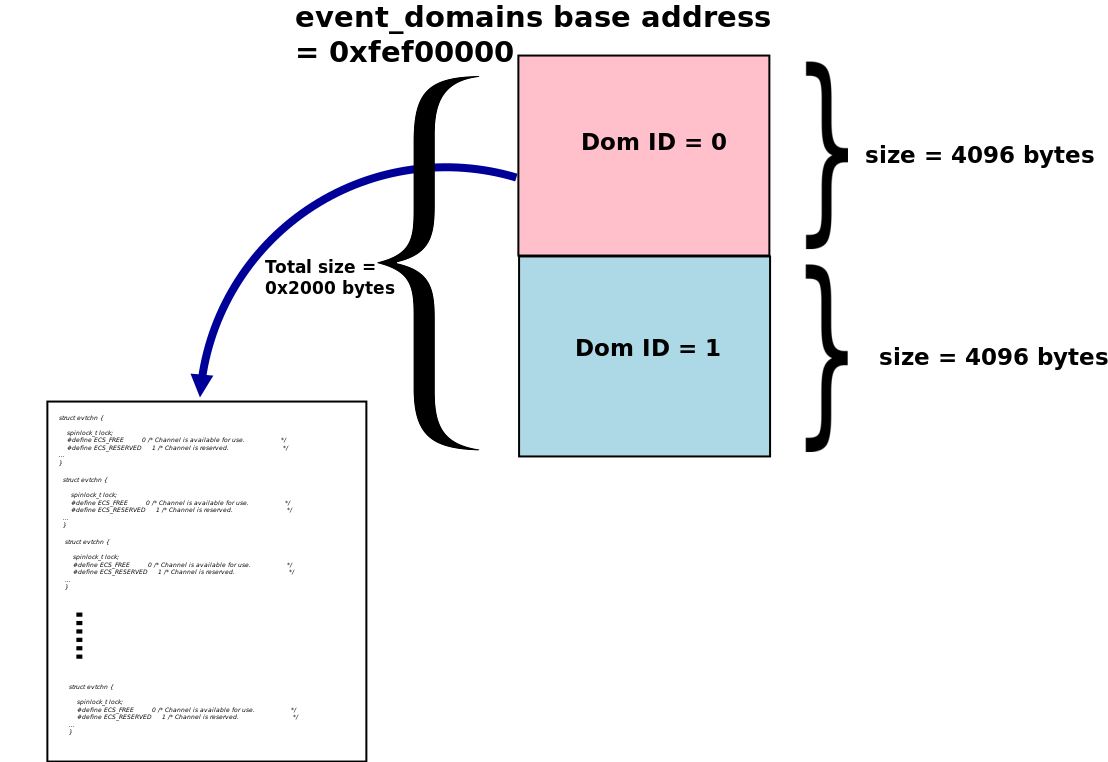
\includegraphics[width=10cm]{event_domains}
	\caption{Basic structure of shared event domains pages in PHIDIAS for two guests}
	\label{event_domains}
\end{figure}

\subsection{Adding Capabilities for IPI in PHIDIAS \label{sec:eventsdomains}}
In Xen split driver model, virtual guests use event channels in two scenarios:
\begin{itemize}
	\item Sending event notifications between Xenstore userspace application and PV I/O drivers, behaving more like an intra-domain event.
	\item Sending event notifications between frontend and backend of split drivers, behaving more like an inter-domain event.
\end{itemize}
For the above two types of events, two capabilities had been added in guest configuration on PHIDIAS as shown in listing \ref{cap}.\\

\begin{lstlisting}[caption=Capabilities added for event notifications in guest configuration on PHIDIAS, label={cap}]
For Dom0 Linux guest 1
      <cap type="ipc" target_xref="linux2" param="0x9" /> 
      <cap type="ipc" target_xref="linux1" param="0x9" /> 
For DomU Linux guest 2
      <cap type="ipc" target_xref="linux1" param="0x9" /> 
      <cap type="ipc" target_xref="linux2" param="0x9" /> 
\end{lstlisting}

Both capabilities had type \textbf{ipc}. First capability had index 0 with destination selected to be remote guest and second capability had index 1 with destination chosen to be itself. First capability was used for \textbf{inter-domain events} and second capability emulated \textbf{intra-domain events}. Both these capabilities triggered SGI 9 for Xen events in virtual guests.

\section{Design of Porting Xenstore\label{sec:xenstorestatic}}
As explained previously in section \ref{sec:xenstore}, each guest in Xen shares a page consisting of ring buffers for requests/responses with Xenstore. It also binds an event channel with Xenstore daemon to send event notifications. A \textbf{\textit{Xen filesystem (xenfs)}} driver is used for creating and mounting files for communication between guests and Xenstore. Out of these files, following two are used for communication between Xenstore and Xen Dom0 guest:
\begin{itemize}
	\item xsd\_kva for mapping Dom0 shared page into Xenstore.
	\item xsd\_port for getting an unbound event channel number of Dom0 used for binding it with an event port in Xenstore daemon. 
\end{itemize}
In native Xen setup, Dom0 creates unprivileged guests and manage them through domain control specific hypercalls. During the process of creating DomU, a Xenstore interface page and an unbound event channel are allocated which are then introduced to Xenstore daemon through Xen's XL tool. Later during initialization, DomU maps this Xenstore interface page into its address space and gets the xenstore event channel number with the help of hypercalls.
\\
\\
In our current work, since no XL tool had been ported and Dom0 did not control creation of DomU guests, DomU Xenstore interface page and event channel number were added manually in Xenstore.For this purpose, a similar file interface as xsd\_kva had been exported to Xenstore daemon by Dom0 used for mapping DomU's Xenstore page as shown in listing \ref{xvd_foreign}. Two globally shared static pages were allocated for implementing Xenstore interfaces of guests in PHIDIAS  as shown in Figure \ref{xenstore-Page}. For event channel of DomU, event port number 1 was hard-coded in Xenstore daemon. DomU had been introduced manually in Xenstore application in file xen/tools/xenstore/xenstored\_domain.c as shown in listing \ref{xenstorelist}.
\\
\\
\begin{lstlisting}[caption=Added file interface for mapping DomU xenstore interface page into userspace in drivers/xen/xenfs/xenstored.c file, label={xvd_foreign},frame=single,style=base]
...
static int @ xsd_foreign_kva_mmap @(struct file *file, struct vm_area_struct *vma)
{
    size_t size = vma->vm_end - vma->vm_start;

    if ((size > PAGE_SIZE) || (vma->vm_pgoff != 0))
        return -EINVAL;
        
    vma->vm_page_prot = pgprot_noncached(vma->vm_page_prot);

    if (io_remap_pfn_range(vma, vma->vm_start,
                           0xfee45000 >> XEN_PAGE_SHIFT,
                           size, vma->vm_page_prot))
        return -EAGAIN; 

    return 0;
}

const struct file_operations xsd_kva_foreign_file_ops = {
    .open = xsd_foreign_kva_open,
    .mmap = @xsd_foreign_kva_mmap@,
    .read = xsd_read,
    .release = xsd_release,
};

...
\end{lstlisting}

\begin{lstlisting}[caption= Manual introduction of DomU in Xenstore during dom0 initialization ,label={xenstorelist}]
static int dom0_init(void) 
{
...
domU = find_domain_by_domid(1);

if (domU == NULL) 
{
/* Hang domain off "in" until we're finished. */
domU = new_domain(dom0->conn->in, 1, 1);
if (!domU) {
return -1;
}
domU->mfn = 0xfee45000 >> 12;
domU->interface = xenbus_map_foreign();
if (domU->interface == NULL) {
return -1;
}

/* Now domain belongs to its connection. */
talloc_steal(domU->conn, domU);

fire_watches(NULL, "@introduceDomain", false);
} 

domain_conn_reset(domU); 
... 
}
\end{lstlisting}

\begin{figure}[!htbp]
	\centering
	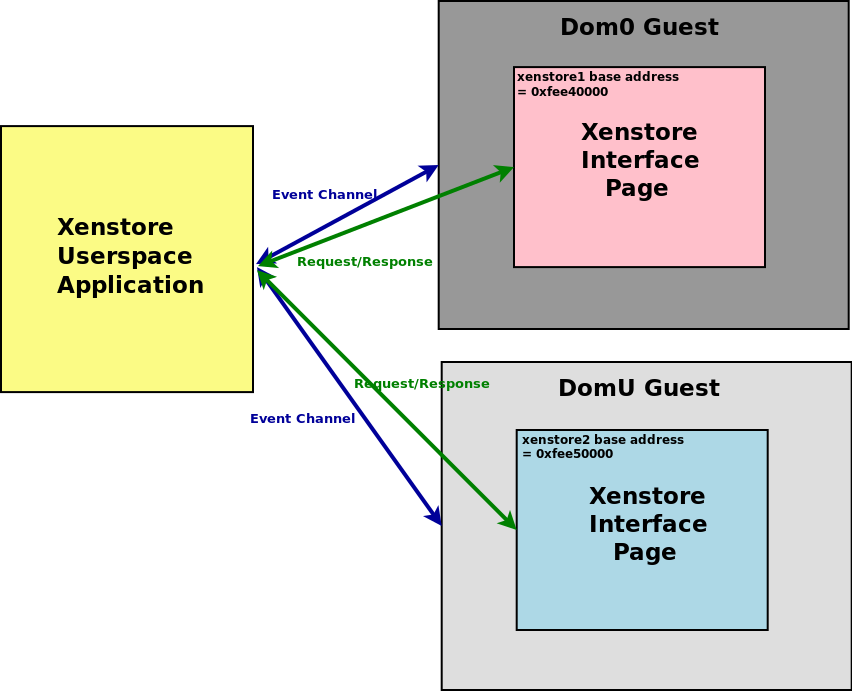
\includegraphics[width=10cm]{xenstore-Page}
	\caption{Communication between Xenstore application and Guests in PHIDIAS}
	\label{xenstore-Page}
\end{figure}


    \chapter{Porting Xen Network Virtualization\label{cha:chapter6}}
In this chapter, first Xen network virtualization architecture will be explained and then the work related to porting it to PHIDIAS will be presented. Other split drivers for different I/O devices can ported using the same approach adopted for paravirtualized network driver with some little modifications corresponding to the requirements for these split drivers.

\section{Xen Network Virtualization \label{sec:xennetwork}}
In this section, analysis of xen network architecture and data flow will be provided. The details of bringing up network virtual interfaces in domains will be explained. Most of the steps performed during registration and initialization of xen network drivers also applies to other I/O virtual drivers of xen. These general steps will also be mentioned in this section.

\section{XenBus Backend and Frontend drivers \label{sec:xenbus}}
All split I/O drivers of Xen depends upon a general bus entity named XenBus which provides an interface to backend and frontend drivers to communicate with each other. The internal working of Xenbus is dependent upon Xenstore and event channels. Xenbus is composed to two parts that work together to provide successful connection of I/O split drivers. These are:
\begin{itemize}
	\item \textbf{XenBus Backend} is a bus that itself is registered with kernel bus subsystem. It is responsible for enumerating all backend devices in Xenstore, calling their corresponding probe functions and watching xenstore for changes. All backend drivers register themselves with XenBus backend.
	\item \textbf{XenBus Frontend} is also a type of bus which registers itself with kernel bus subsystem. It is responsible for enumerating and probing all frontend devices in Xenstore and registering watches in Xenstore for getting notification about changes in the backend devices. All frontend drivers registert themselves with XenBus frontend.
\end{itemize}
    \chapter{Testing and Evaluation\label{cha:chapter7}}
In this chapter, results of tests performed for comparing network performance on Xen and PHIDIAS will be presented and analyzed. Two tests were performed for calculating statistics on network performance on Xen and PHIDIAS. One test was conducted to calculate the latency of transferring network packets between Dom0 and DomU and the second one was done to measure throughput. Both tests were performed by running two Linux guests on different physical CPU cores on an 8-core Hikey ARMv8 target platform. Analysis and results of these tests are presented in following sections.

\section{Network Latency Test \label{sec:testenv}}
Ping is the most common utility to measure round trip latency of network packets. For our tests, Ping binary used was of \textbf{BusyBox v1.22.1 (Debian 1:1.22.0-9+deb8u1) multi-call binary}. Ping utility was obtained from prebuilt binary of ramdisk image of 96boards' linaro debian at web link \cite{initrd}.
\\
\\
Ping tests were performed with different packet sizes using default Ethernet maximum transmission unit (MTU) i.e. 1500 bytes.  Each test was conducted for 50 packets and then minimum, average and maximum round trip latencies were calculated. For TCP/IP networking, if network packet size is larger than MTU, IP fragmentation occurs \cite{frag}. For testing fragmentation in our setup, packet size of 1900 bytes was used.

\subsection{Network Latency Test results on Xen \label{sec:testlatencyxen}}
Table \ref{ping_xen} shows the results of ping tests performed between Dom0 and DomU through virtual network devices on Xen.

\begin{table}[htbp]
	\caption{Ping Test results on Xen}
    \centering
	\resizebox{\textwidth}{!}{\begin{tabular}{|r|l|r|r|r|r|l|}
		\hline
		\multicolumn{1}{|l|}{\textbf{Number of packets}} & \textbf{Size of data in Bytes} & \multicolumn{1}{l|}{\textbf{Min RTT (ms)}} & \multicolumn{1}{l|}{\textbf{Avg RTT (ms)}} & \multicolumn{1}{l|}{\textbf{Max RTT (ms)}} & \multicolumn{1}{l|}{\textbf{Packets Lost}} & \textbf{Reason} \\ \hline
		50 & 56 (default) & 0.42 & 0.533 & 0.718 & 0 & N/A \\ \hline
		50 & 1000 & 0.402 & 0.611 & 0.857 & 0 & N/A \\ \hline
		50 & 1900 (with fragmentation) & 0.483 & 0.699 & 0.913 & 0 & N/A \\ \hline
	\end{tabular}}
	\label{ping_xen}
\end{table}


\subsection{Network Latency Test results on PHIDIAS \label{sec:testlatencyphidias}}
Table \ref{ping_phidias} shows the results of ping tests performed between Dom0 and DomU through virtual network devices on PHIDIAS.

\begin{table}[htbp]
	\caption{Ping Test Results on PHIDIAS}
	 \centering
	\resizebox{\textwidth}{!}{\begin{tabular}{|r|l|r|r|r|r|l|}
		\hline
		\multicolumn{1}{|l|}{\textbf{Number of packets}} & \textbf{Size of data in Bytes} & \multicolumn{1}{l|}{\textbf{Min RTT (ms)}} & \multicolumn{1}{l|}{\textbf{Avg RTT (ms)}} & \multicolumn{1}{l|}{\textbf{Max RTT (ms)}} & \multicolumn{1}{l|}{\textbf{Packets Lost}} & \textbf{Reason} \\ \hline
		50 & 56 (default) & 0.135 & 0.147 & 0.36 & 0 & N/A \\ \hline
		50 & 1000 & 0.234 & 0.251 & 0.558 & 0 & N/A \\ \hline
		50 & 1900 (with fragmentation) & 0.394 & 0.407 & 0.427 & 30 & IP reassembly Timeout \\ \hline
	\end{tabular}}
	\label{ping_phidias}
\end{table}

\subsection{Analysis of Network Latency Test results on PHIDIAS \label{sec:testlatencyeval}}

Figure \ref{ping_rtt} shows the comparison between round trip latencies of ping packets on PHIDIAS and Xen. It is clear that PHIDIAS outperforms Xen with lower latencies. This is due to the fact that no hypercalls and switching into hypervisor world is done in case of network virtualization on PHIDIAS. PHIDIAS does all the static allocations and configurations at compile time and the guests are then responsible for transferring network packets by sharing and mapping pages into their corresponding address spaces.


\section{Network Throughput Test \label{sec:testenvthrough}}

\subsection{Network Throughput Test results on Xen \label{sec:testthroughxen}}

\subsection{Network Throughput Test results on PHIDIAS \label{sec:testthroughphidias}}

\subsection{Analysis of Network Throughput Test results on PHIDIAS \label{sec:testthrougheval}}
    \chapter{Conclusion and Future Work\label{cha:chapter8}}

\section{Conclusion \label{sec:Conclusion}}
This thesis explains the necessary background details required for porting Xen I/O virtualization architecture onto PHIDIAS. Modifications for porting dynamic components of Xen split driver model to a statically configured hypervisor are discussed. This includes required changes for all paravirtualized I/O drivers of Xen in general and for virtual network devices in particular. Tests network performance comparison on Xen and PHIDIAS have shown that ported virtual network drivers on PHIDIAS outperform Xen for packets of sizes smaller than default Ethernet MTU size. Performance degradation happens only for fragmented packets which occurs due to overhead of two additional memory copy operations on statically shared un-cached memory pages between guests on PHIDIAS. In the current implementation strategy of porting, a simpler approach has been adopted with less changes overall but it has caused lower performance for fragmented network packets.
\\
\\
This work has contributed to the extension of PHIDIAS functionality regarding support of I/O virtualization. 
Keeping changes in both Xen paravirtualized I/O drivers and PHIDIAS hypervisor to a minimum has served two purposes. First, it has proved the flexibility of PHIDIAS static design and kept its integrity proof by symbolic execution valid. Second, it has enabled to reuse the maintenance support of Xen community.

\section{Future work \label{sec:Futurework}}
There are still several enhancements that could be performed to expand the feature set of PHIDIAS. It includes passing-through of physical network devices (WLAN and USB-Ethernet) on HiKey ARMv8 target to domain0 in order to talk to outside world and porting Xen I/O drivers for x86 target to PHIDIAS.
\\
\\
The main goal of this thesis is to provide a proof-of-concept for working I/O split driver of Xen on PHIDIAS. It has achieved this purpose by running logical network devices on virtual machines on top of PHIDIAS. However, lower performance for fragmented packets was obtained for throughput tests. In order to improve performance, method that was used for transmission of packets from netfront to netback in this work could be re-designed. 


init_mm.pgd
create_pgd_mapping
move_ptes

instead of copying entire pages of 4KB (or 2MB for huge pages), we are swapping integers inside the kernel structure
we are touching hot structures in the kernel, neither cold memory, nor bytes swapped on disk\textbf{}
Redesigning mapping operations in netback receive path for faster network operations


Deployment in high end embedded systems for comparing Xen and PHIDIAS

% ---------------------------------------------------------------
\backmatter % no page numbering from here
   % \addchap{List of Acronyms}

\begin{tabbing}

\end{tabbing}
\endinput

		
		% if you want to provide a glossary with explanations of important terms put it in here

    \bibliographystyle{ieeetr}
    \bibliography{./bib/references}
    
    %\addchap{Annex}

\begin{appendix}

\lstset{language=,caption=Sourcecode Listing,captionpos=b,
label=yahoowidgetkon,showstringspaces=false,
basicstyle={\fontfamily{pcr}\selectfont\footnotesize}}
\begin{lstlisting}
<?xml version="1.0" encoding="UTF-8"?>
<widget>
	 <debug>off</debug>
	 <window name="myWindow" title="Hello Widget" visible="true">
		 <height>120</height>
		 <width>320</width>
		 <image src="Resources/orangebg.png">
			<name>orangebg</name>
			<hOffset>0</hOffset>
			<vOffset>0</vOffset>
		</image>
		 <text>
			 <name>myText</name>
			 <data>Hello Widget</data>
			 <color>#000000</color>
			 <size>20</size>
			 <vOffset>50</vOffset>
			 <hOffset>120</hOffset>
		 </text>
	</window>
</widget>
\end{lstlisting}

\newpage


\lstset{caption=SIP request and response packet\cite{SIPBook},
captionpos=b,label=sippacket,showstringspaces=false,
basicstyle={\fontfamily{pcr}\selectfont\footnotesize}}
\begin{lstlisting}
INVITE sip:bob@network.org SIP/2.0
Via: SIP/2.0/UDP 100.101.102.103:5060;branch=z9hG4bKmp17a
Max-Forwards: 70
To: Bob <sip:bob@network.org>
From: Alice <sip:alice@ims-network.org>;tag=42
Call-ID: 10@100.101.102.103
CSeq: 1 INVITE
Subject: How are you?
Contact: <sip:xyz@network.org>
Content-Type: application/sdp
Content-Length: 159
v=0
o=alice 2890844526 2890844526 IN IP4 100.101.102.103
s=Phone Call
t=0 0
c=IN IP4 100.101.102.103
m=audio 49170 RTP/AVP 0
a=rtpmap:0 PCMU/8000

SIP/2.0 200 OK
Via: SIP/2.0/UDP proxy.network.org:5060;branch=z9hG4bK83842.1
;received=100.101.102.105
Via: SIP/2.0/UDP 100.101.102.103:5060;branch=z9hG4bKmp17a
To: Bob <sip:bob@network.org>;tag=314159
From: Alice <sip:alice@network.org>;tag=42
Call-ID: 10@100.101.102.103
CSeq: 1 INVITE
Contact: <sip:foo@network.org>
Content-Type: application/sdp
Content-Length: 159
v=0
o=bob 2890844526 2890844526 IN IP4 200.201.202.203
s=Phone Call
c=IN IP4 200.201.202.203
t=0 0
m=audio 49172 RTP/AVP 0
a=rtpmap:0 PCMU/8000
\end{lstlisting}


\end{appendix}

\endinput


\end{document}
